% Manuscript draft -- Havana Bay: robust vs fragile conclusions about flushing
% Target: Environmental Modelling & Software (Elsevier), research article.
% Class: elsarticle (official: github.com/STM-Document-Engineering/elsarticle, 04aee43).
% EMS rules (Guide for Authors, checked 17-oct-2026): abstract <= 150 words;
% 1-7 keywords; 3-5 highlights of <= 85 characters (separate file at submission);
% graphical abstract required; data deposited in a repository and cited;
% CRediT, competing interests, funding and GenAI declaration required.
%
% RULE: every input is public and replicable. Unpublished data (CUJAE, GEOCUBA,
% tide-gauge series) may only appear as optional comparison.
% Numbers: source of truth is repos/Modelo-hidrodin-mico/docs/articulo/cifras.md
% (state of 8-nov-2026, commit 1e32fcf of the working repo).
% \prov{} = provisional value (blue); \todo{} = missing content (red).
% 14-nov: rewritten for focus (6 figures, 5 tables); removed figures stay in figuras/.
% 14-nov (review V1): headline aligned on 'one to two weeks'; tracer-protocol deviation
% declared; pilot depth and 2002 river data attributed as in the sources; DOIs completed.
% 16-nov (review V2): reframed around parametric vs structural uncertainty; heat-flux
% results moved to the centre (Fig. 7, Table 4 column); Sentinel-2 figure in main text;
% mesh, tide check and tidal prism figures added to the supplement; numerical behaviour
% moved to Text S1; Table 2 gains a 'Basis' column; unused affiliations removed.
% 17-nov (review V3, mode 'full'): new title; results reordered (heat flux right after
% Sobol, then its seasonal behaviour, then rivers); thermal-brake hypothesis in Discussion
% (Largier 2010; Monismith 2006); claims matched to evidence (peer-review claim matrix).
% fig_heatflux.pdf was cropped from Alex's compiled PDF of 17-nov (not in the zip).
% 17-nov (V3, second pass): prose rewritten for flow and length (~6900 -> ~5300 words of
% prose); 18 -> 13 headings; question list and numbered conclusions turned into prose;
% tracer, Sentinel-2 and numerical details moved to Texts S1-S3.
\documentclass[a4paper,fleqn]{ems-dc}
\usepackage[authoryear]{natbib}
\usepackage{graphicx}
\usepackage{booktabs}
\usepackage{xcolor}
\usepackage{enumitem}
%\usepackage[section]{placeins}
%\usepackage{lineno}\linenumbers   % line numbers for review: uncomment
\setlength{\emergencystretch}{2em}
\setlength{\tabcolsep}{4pt}
\AtBeginEnvironment{table}{\small}
\AtBeginEnvironment{table*}{\small}
\newcommand{\todo}[1]{\textcolor{red}{[TODO: #1]}}
% Placeholder for a link Alex fills in (red, typewriter): replace the whole \ph{...}.
\newcommand{\ph}[1]{\textcolor{red}{\textsf{#1}}}
\newcommand{\prov}[1]{\textcolor{blue}{#1}}

\begin{document}
\let\WriteBookmarks\relax
\shorttitle{Flushing of Havana Bay from public data}
\shortauthors{A.M. Rivera-Rivera et al.}

\title[mode=title]{When model structure matters as much as the data: water renewal in Havana Bay, Cuba, from public-data ensembles}

\author[1,2,3]{Alex M. Rivera-Rivera}
\cormark[1]
\ead{alex.rivera.rivera@ulb.be}
\credit{Conceptualization, Data curation, Formal analysis, Investigation, Methodology,
Resources, Software, Validation, Visualization, Writing -- original draft, Writing --
review \& editing}
\author[3,2]{Daniela Martinez-Ortiz}
\credit{Conceptualization, Data curation, Formal analysis, Investigation, Methodology,
Resources, Software, Validation, Visualization, Writing -- original draft, Writing --
review \& editing}
\author[3]{Ernesto Altshuler}
\credit{Conceptualization, Investigation, Methodology, Project administration,
Supervision, Writing -- review \& editing}
\author[4]{Alexandre Campo}
\credit{Conceptualization, Formal analysis, Investigation, Methodology, Visualization,
Writing -- review \& editing}
\author[4]{Stamatios C. Nicolis}
\credit{Conceptualization, Formal analysis, Investigation, Methodology, Project
administration, Supervision, Visualization, Writing -- review \& editing}

\affiliation[1]{organization={Innovation Laboratory, Technological University of Havana Jos\'e Antonio Echeverr\'ia (CUJAE)},
  postcode={19390}, city={Havana}, country={Cuba}}
\affiliation[2]{organization={Facult\'e des Sciences, Universit\'e Libre de Bruxelles (ULB)},
  postcode={1050}, city={Brussels}, country={Belgium}}
\affiliation[3]{organization={Center for Complex Systems, Physics Faculty, University of Havana},
  postcode={10400}, city={Havana}, country={Cuba}}
\affiliation[4]{organization={Brussels School of Engineering, Universit\'e libre de Bruxelles},
  addressline={Avenue Franklin Roosevelt 50}, postcode={1000}, city={Brussels}, country={Belgium}}
\cortext[1]{Corresponding author}
% Authors, affiliations, CRediT roles, funding and AI statement as in the FocalReview
% manuscript (Alex, 13-nov-2026); author list as in the V2 received on 16-nov-2026.

% <= 150 words (16-nov).
\begin{abstract}
Many polluted bays lack the surveys, tide and current records to calibrate a hydrodynamic
model. We ask which conclusions about their flushing survive without them. Havana Bay (Cuba),
a 4.9~km$^2$ bay behind a 1.5~km channel, is modelled in 3D with SCHISM from public data
only; nine poorly known inputs, from nineteenth-century charts to river discharge, are
sampled in a 704-member Sobol ensemble. The tide alone renews the bay poorly; an estuarine
circulation driven by 2~m$^3$\,s$^{-1}$ of river water does. In the dry season the
bay-mean water age is 7.8~days (5.6--10.4, 90\% range) and depends mostly on river
discharge. Adding the air--sea heat flux, left out of the ensemble, raises it in all 64
members tested, to a median of 13.2~days: a shift as large as the whole spread caused by the
nine inputs. The bay is renewed in one to two weeks, not months.
\end{abstract}

% Highlights: 3-5 items, each <= 85 characters; also submitted as a separate file.
\begin{highlights}
\item A 3D model of Havana Bay built from public data only, run as a 704-member ensemble.
\item An estuarine circulation driven by the rivers, not the tide, renews the bay.
\item River discharge controls most of the uncertainty that comes from the inputs.
\item Adding the air--sea heat flux raises the age in all 64 members tested, to two weeks.
\item One structural choice shifts the age as much as all nine sampled inputs together.
\end{highlights}

\begin{keywords}
water age \sep residence time \sep ensemble modelling \sep global sensitivity analysis \sep
structural uncertainty \sep historical nautical charts \sep Havana Bay
\end{keywords}

\maketitle

%======================================================================
\section{Introduction}\label{sec:intro}
%======================================================================
Semi-enclosed bays collect the waste of the cities around them, and how long their water
stays inside goes a long way towards deciding how much of that load becomes a water-quality
problem. Flushing time, residence time and water age are the usual ways of putting a number
on this \citep{Monsen2002,Deleersnijder2001,Lucas2020}. Computing them well normally
requires a calibrated hydrodynamic model, and calibration requires bathymetry, water levels
and currents that many bays in the Global South simply do not have. Recent work has
therefore built such models from satellite and reanalysis data alone \citep{Payandeh2026},
or calibrated them on a handful of measurements \citep{RodriguesDoAmaral2025}.

Faced with missing data, the usual course is to build one model from whatever can be found
and to report one residence time. That number is hard to defend, because it carries every
guess made along the way and the reader cannot tell which conclusion rests on which guess
\citep{Uusitalo2015}. A variance-based sensitivity analysis over a large ensemble
\citep{Sobol2001,Saltelli2008,Saltelli2010} helps, since it explores all uncertain inputs
together rather than one at a time \citep{Saltelli2019,Pianosi2016,Razavi2021}. But it only
explores the inputs of one model. Processes that the model leaves out, or represents too
simply, are a separate source of uncertainty that no amount of input sampling will reveal
\citep{Walker2003,Refsgaard2006,Gupta2012}.

Havana Bay shows why this matters. Its sediments record metal pollution
\citep{DiazAsencio2011} and its benthic fauna lives under chronic, heavy pollution
\citep{Armenteros2009}, yet, to our knowledge, it has been modelled only for coastal flooding
and wave overtopping along the Malec\'on \citep{PoncePortela2012,CordovaDeHorta2025}, and no
peer-reviewed study has quantified how its water is renewed. The one figure in circulation,
a freshwater retention time of about four months with little exchange with the sea, comes
from the executive summary of a sewerage master plan that does not say how it was obtained
\citep{JICA2004}. The only open bathymetry inside the bay comes from two nineteenth-century
editions of a single nautical chart.

We set out to learn what can be said about the renewal of this bay from public data alone,
and how firmly. The first step is to find out what drives the exchange with the sea: the
tide, the wind or the density contrast created by the rivers. We then sample every poorly
known input in a 704-member Sobol ensemble, which tells us how long water stays in each part
of the bay, which of those answers survive the missing data, and which unknown matters most
and should be measured first. Finally, we step outside the ensemble and change the model
itself. The most consequential of these changes turned out to be the air--sea heat flux,
which in bays with little river inflow can shape the density contrast with the sea as much
as fresh water does \citep{Largier2010}. Adding it moves the answer as far as all nine
sampled inputs together. That result matters beyond Havana Bay, because it shows in numbers
how the spread of a parametric ensemble can understate the uncertainty when a structural
choice is left out of it. Every input is public and the code is open, so the procedure can
be repeated in other bays that have no surveys or gauges.

%======================================================================
\section{Study area and data}\label{sec:area}
%======================================================================
Havana Bay (Fig.~\ref{fig:map}) is a pocket bay of 4.91~km$^2$, connected to the sea by an
entrance channel 1530~m long and 220--330~m wide that opens to the north-west and is 12.8~m
deep according to the harbour pilots \citep{Practicos2018}. Behind the channel lies a main
basin 9--13~m deep, and from it branch three coves, mostly shallower than 4~m on the
historical charts: Marimelena to the east, Guasabacoa to the south and Atar\'es to the
south-west. Depending on how much of the dredging reported by the pilots is applied, the bay
holds 26--36~hm$^3$ (Section~\ref{sec:bathy}); the often quoted mean depth of 9~m and volume
of 47~hm$^3$ \citep{JICA2004} agree with neither the charts nor the pilots' depths.

\begin{figure*}[!t]
\centering
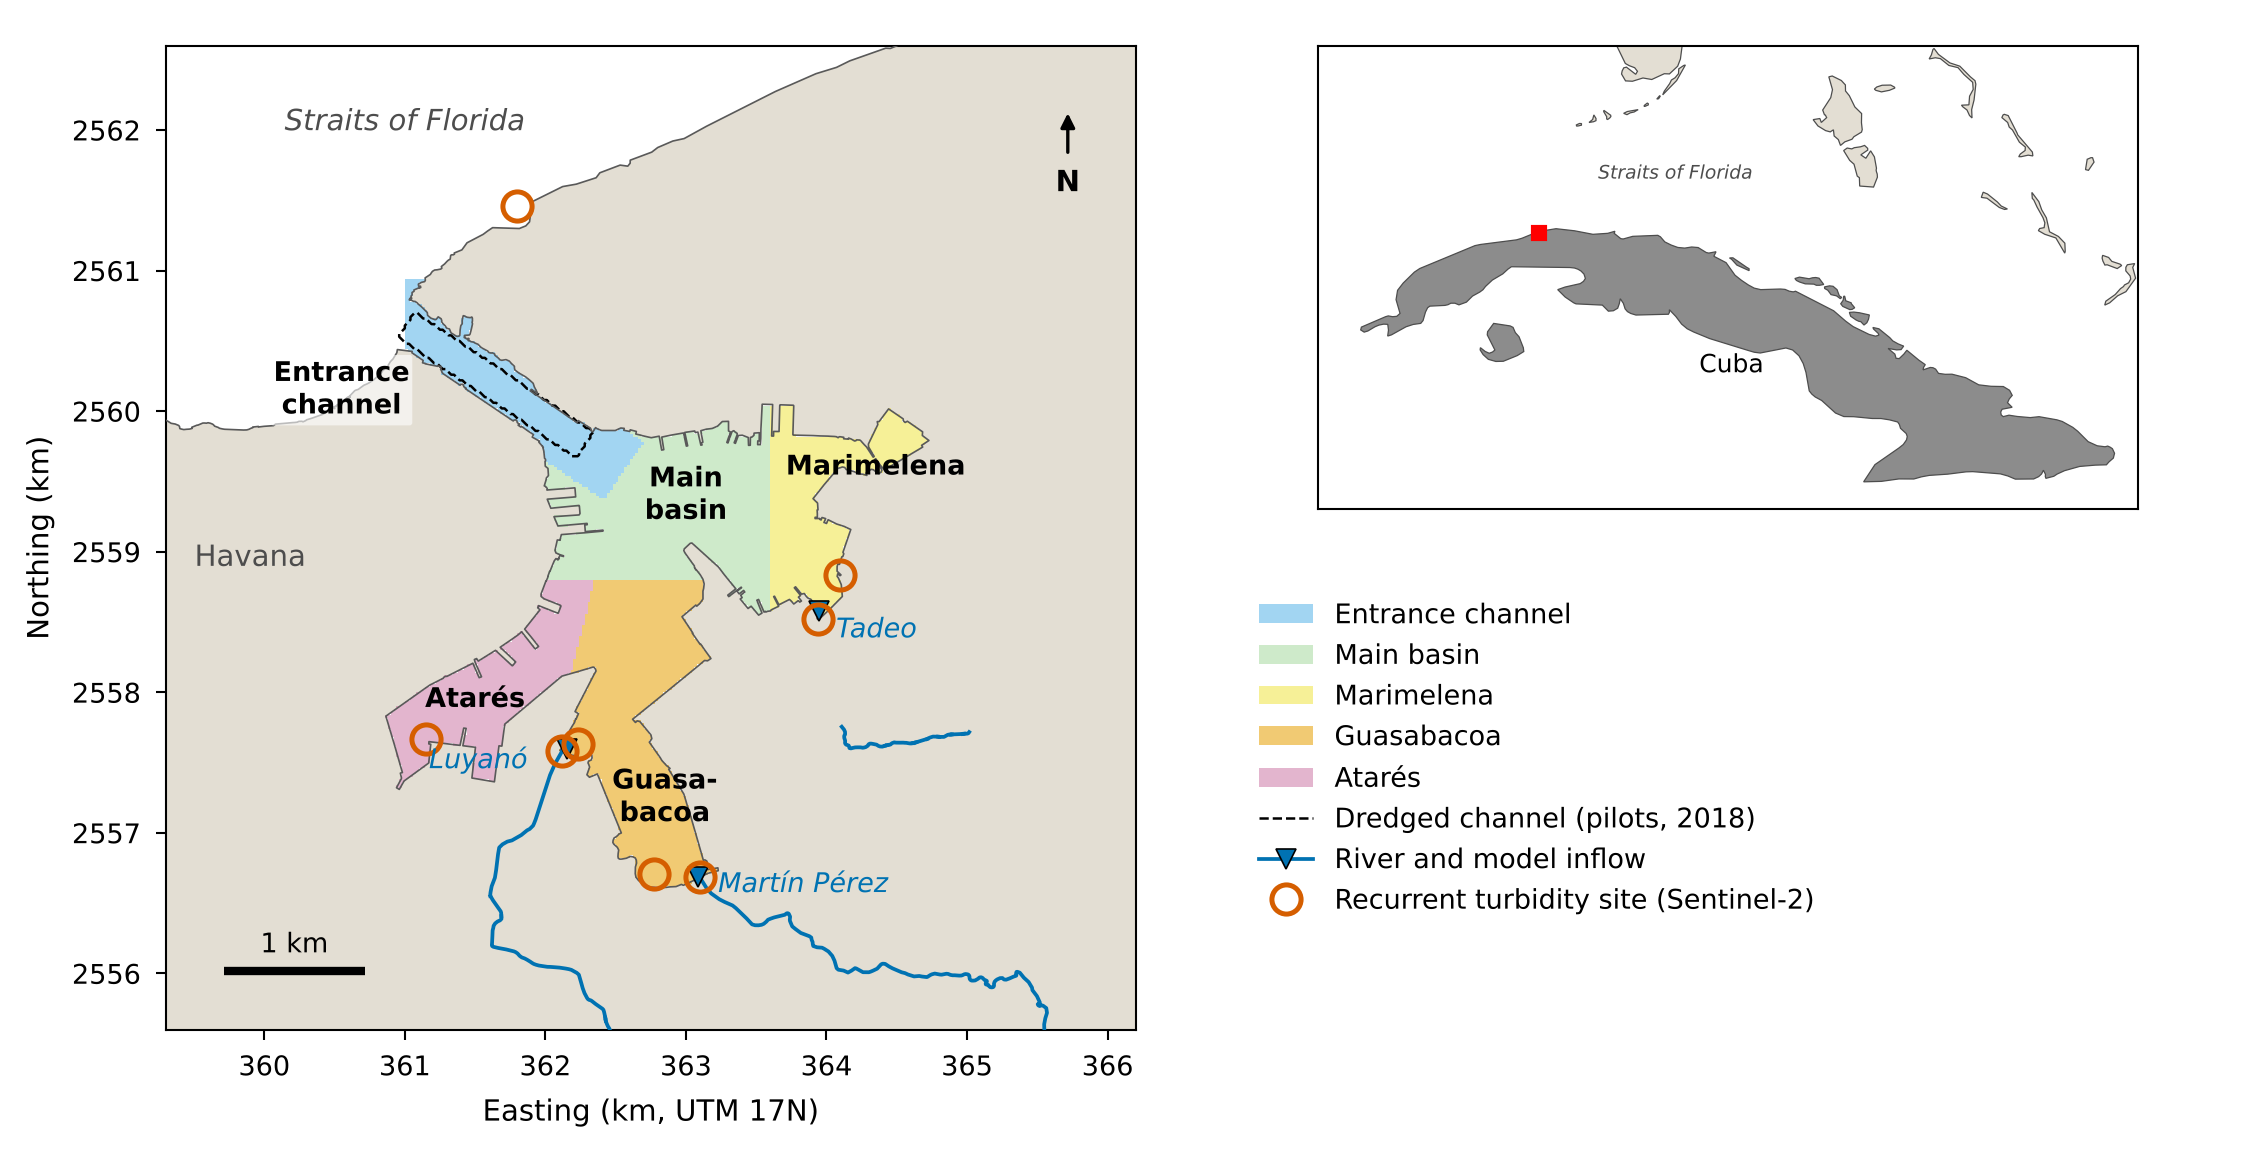
\includegraphics[width=\textwidth]{figuras/fig01_map.png}
\caption{Havana Bay: entrance channel, main basin, coves, river mouths and the five
analysis zones. Orange circles mark the foci listed by the Sentinel-2 study
(\ph{link\_sentinel2}): one preregistered candidate site (entrance channel), three
exploratory foci chosen after seeing the data, and four river or drain mouths from
OpenStreetMap; none is a validated discharge site. Blue triangles are the model river
inflows. The dashed outline is the channel dredged to the depth reported by the harbour
pilots \citep{Practicos2018}. Inset: location in Cuba (Natural Earth, public domain). Map
lines delineate study areas and do not necessarily depict accepted national
boundaries.}\label{fig:map}
\end{figure*}

The tide is small and mixed, as in much of the Caribbean \citep{Kjerfve1981}. Off the mouth,
two independent global models give M2 amplitudes of 12.2 and 12.6~cm, K1 of 8.3 and 8.0~cm
and O1 of 8.8 and 8.4~cm \citep{FES2022,HartDavis2021}, so diurnal and semidiurnal
constituents are of similar size (form factor $(K_1+O_1)/(M_2+S_2)$ of 1.0--1.05;
\citealt{Pugh2014}), and the mean range is about 0.29~m \citep{JICA2004}. Three rivers bring
fresh water: the Luyan\'o (1.33~m$^3$\,s$^{-1}$) and the Mart\'in P\'erez
(0.72~m$^3$\,s$^{-1}$) into Guasabacoa, and the Arroyo Tadeo (0.09~m$^3$\,s$^{-1}$) into the
southern shore of Marimelena. These 2.14~m$^3$\,s$^{-1}$ are a single set of values dated
August 2002 (CIMAB) and reported by \citet{JICA2004}; none of the rivers is gauged. No river
reaches Atar\'es in OpenStreetMap, although drains discharge there, and urban and industrial
sewage adds a load that nobody has quantified \citep{JICA2004}.

Every input is public (Table~\ref{tab:data}), and none requires an agreement, a purchase or
a personal contact. FES2022, which needs a free account, is used only as a check; the
simulations are forced with EOT20, which needs no registration. Each download is logged with
its date and checksum in the code repository.

\begin{table*}[!t]
\centering\small
\caption{Inputs of the model and of its evaluation. All are public.}\label{tab:data}
\begin{tabular}{p{3.0cm}p{9.8cm}p{4.0cm}}
\toprule
Input & Source & Role\\
\midrule
Bathymetry inside the bay & U.S. Hydrographic Office chart No.~307, \emph{Harbor of
Havana}, from Spanish surveys to 1879 (ed.~1889) and to 1887 (ed.~1898)
\citep{USHO1889,USHO1898}; 1126 and 1514 digitised soundings & Ensemble input\\
Entrance channel and quays & Harbour-pilot depths \citep{Practicos2018} & Dredging state\\
Offshore bathymetry & GEBCO 2026 grid \citep{GEBCO2026} & Outer domain\\
Coastline, river mouths & OpenStreetMap \citep{OSM} & Fixed\\
Atmosphere & ERA5 hourly, 2016--2025 \citep{Hersbach2020} & Forcing; wind perturbed\\
Tide & EOT20, 9 constituents \citep{HartDavis2021} & Boundary; amplitude perturbed\\
Tide (comparison) & FES2022, 11 constituents \citep{FES2022,Lyard2026} & Check of EOT20\\
River flows & Values of August 2002 (CIMAB), in \citet{JICA2004} & Ensemble input\\
Sea-surface temperature & NOAA OISST v2.1, daily \citep{Huang2021} & Structural tests\\
Turbidity persistence & Sentinel-2, 2017--2025 (\ph{link\_sentinel2}) & Evaluation only\\
Model & SCHISM \citep{Zhang2016} & Open source\\
\bottomrule
\end{tabular}
\end{table*}

%======================================================================
\section{Methods}\label{sec:methods}
%======================================================================
\subsection{Bathymetry from nineteenth-century charts}\label{sec:bathy}
The two editions of chart No.~307 record independent Spanish surveys of the bay, one
completed in 1879 and the other in 1887. Lead-line soundings of this kind have been used to
reconstruct past bathymetry and to model how estuaries change
\citep{Jaffe2007,Ralston2019,Poirier2020}. We digitised them by hand
(Fig.~\ref{fig:soundings}), converting fathoms to metres, from a georeferenced scan of the
1889 edition (RMS error 18~m) and from the 1898 edition registered onto it (median residual
1.2~m), and interpolated them onto a 20~m UTM grid, with the OpenStreetMap coastline at zero
depth and GEBCO blended in 150--600~m away from the nearest sounding. The charts do not state
their vertical datum, so it enters the ensemble as an uncertain offset of 0 to +0.5~m.

Where the two surveys overlap, they tell us how good they are. Their differences show no bias
and a mean absolute value of 0.76~m, and a variogram fitted to 12\,134 of them describes a
spatially correlated error \citep{Plant2002,Cea2012} with $\sigma = 0.9$~m and a correlation
length $L = 150$~m. Each ensemble member receives a Gaussian random field with these
properties, taken from the data rather than assumed; the field fades towards the shore and
leaves the maintained channel untouched.

The bay has been dredged since the surveys, and dredging can change the dynamics of an
estuary substantially \citep{Ralston2019}. A dredging state $\alpha$ between 0 and 1
therefore moves each member from the chart as surveyed ($\alpha = 0$) to a present-day
estimate ($\alpha = 1$), in which the entrance channel is at least 12.8~m deep along its
220~m~$\times$~1530~m alignment and the historically navigable water (at least 5~m deep and
connected to the channel) is 11~m deep, within the 9.75--11.58~m given by the pilots
\citep{Practicos2018}. The bay volume then spans 26--36~hm$^3$, whereas the random field
adds only $\pm 1$~hm$^3$ (Fig.~\ref{fig:bathy}).

\begin{figure*}[!t]
\centering
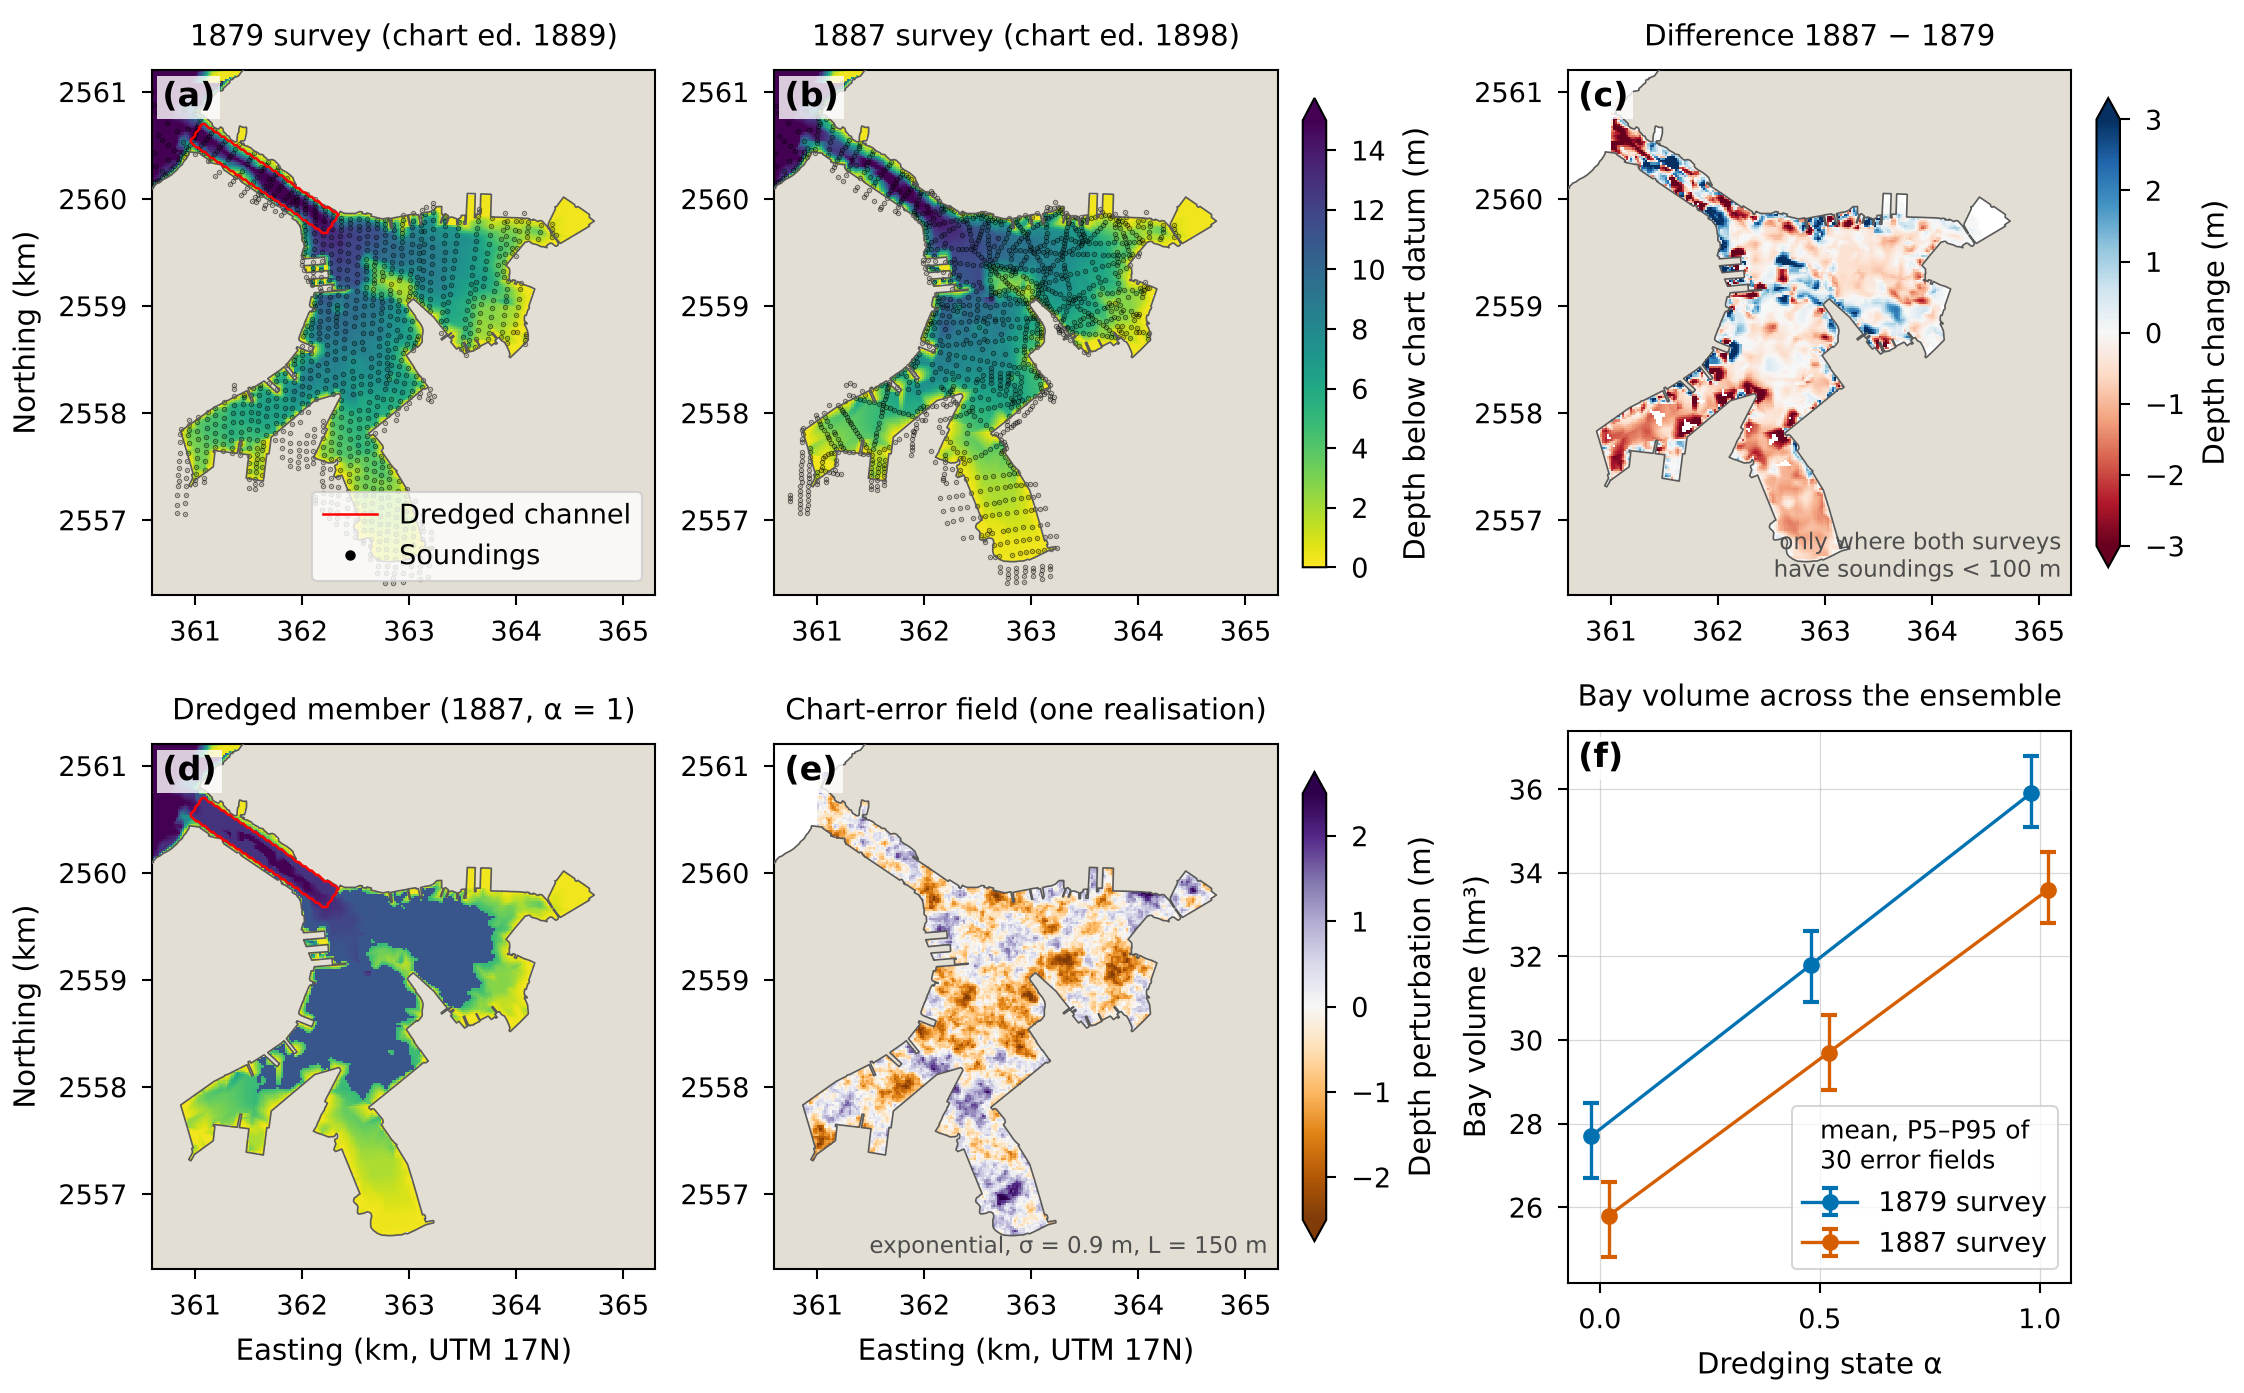
\includegraphics[width=\textwidth]{figuras/fig02_bathymetry.png}
\caption{Bathymetry from chart No.~307 and its uncertainty. (a, b) Interpolated surfaces
and soundings of the 1879 survey (chart edition of 1889) and of the 1887 survey (edition of
1898); the red rectangle is the dredged channel. (c) Difference between the surveys, shown
only where both have soundings within 100~m. (d) Ensemble member with the 1887 survey and
the dredged state ($\alpha=1$). (e) One realisation of the chart-error field. (f) Bay volume
against dredging state for both surveys (mean and P5--P95 of 30 error
fields).}\label{fig:bathy}
\end{figure*}

\subsection{Model, forcing and water age}\label{sec:model}\label{sec:metrics}
We use SCHISM \citep{Zhang2008,Zhang2016} (commit 09f407e8) in three dimensions, with 16
terrain-following levels, a 100~s time step, the $k$--$kl$ form of the generic length-scale
turbulence closure \citep{Umlauf2003,Warner2005} and Coriolis forcing. The unstructured mesh,
built with DistMesh \citep{Persson2004} on a 5~km circle centred on the bay mouth, has 4832
nodes and 8941 triangles, from 25~m in the entrance channel (about 11 elements across it)
and 40~m in the bay to 400~m offshore (Fig.~\ref{fig:mesh}). Its open boundary is a 33-node
arc in 46--1220~m of water. Near that boundary, momentum advection is switched off within
800~m, a friction sponge ($C_d \to 0.05$) acts within 1~km and the wind stress is ramped up
over 2~km; removing the sponge doubled the velocities at the boundary but left levels and
currents inside the bay unchanged to the first decimal.

Hourly ERA5 wind, pressure, air temperature, humidity, radiation and precipitation drive the
surface \citep{Hersbach2020}. ERA5 has only $3 \times 4$ grid points over the area and known
biases in its surface winds \citep{BelmonteRivas2019}, which is why wind speed and direction
are perturbed in the ensemble. The tide at the open boundary is built from the nine EOT20
constituents with nodal corrections \citep{Pugh2014}; FES2022 differs from it by at most
0.4~cm in every constituent amplitude off the mouth and by 1.15~cm RMS in predicted water
level (Fig.~\ref{fig:tide}), well inside the $\pm10\%$ amplitude range of the ensemble. The
rivers enter at the mesh elements nearest their OpenStreetMap mouths. In the ensemble,
density depends on salinity only: river water enters fresh, the open boundary is held at a
salinity of 36 and a temperature of 28~$^\circ$C, and there is no air--sea heat flux,
evaporation or precipitation. All runs start on 1 January 2016 and cover the dry season; the
year was chosen without a particular criterion, after a first look at the 2016--2025 ERA5
period and before any ensemble member was run.

Water age is computed with the age tracer of \citet{Deleersnijder2001} \citep[see
also][]{Delhez1999} as implemented in SCHISM, an approach widely used in estuaries
\citep{Shen2004}, following the definitions of \citet{Monsen2002}. Sea water and river water
both enter with age zero, so age is the time since the water entered the bay by either
route; it is not a freshwater retention time. For comparison with the only earlier estimate,
the few runs that keep full output fields also give the freshwater flushing time
$T_f = V_f/Q$ \citep{Alber1999,Sheldon2002}, where $V_f$ is the fresh water in the bay, from
$1 - S/36$, and $Q$ the river discharge. Each 120-day member is summarised by the
volume-weighted mean age over its last 30 days, in the whole bay and in five zones
(Fig.~\ref{fig:map}: channel, main basin, Marimelena, Guasabacoa and Atar\'es), from fields
written every 4~h. A member is in equilibrium if its bay-mean age changes by at most 0.05~d per day over
its last 10 days; with the air--sea heat flux the forcing changes too much for that
criterion to make sense, and we report 30-day means and their range instead. The discharge
through the channel is computed but not used, because from 4-hourly velocities its net value
carries an error of about $\pm 6$~m$^3$\,s$^{-1}$, more than the river inflow.

\subsection{The ensemble and the conclusions fixed in advance}\label{sec:ensemble}
Nine uncertain inputs (Table~\ref{tab:params}) are sampled with a Saltelli design
\citep{Saltelli2002} on a randomised Sobol sequence; with a base sample of $N = 64$ and
$d = 9$ inputs this gives $N(d+2) = 704$ members of 120 days. That length comes from the
mechanism runs, in which the bay-mean age with rivers settles after about 30 days, and
leaves room for members with little river water. First-order ($S_1$) and total ($S_T$) Sobol
indices are estimated with the Jansen estimators \citep{Jansen1999,Saltelli2010}, with 95\%
intervals from 1000 bootstrap resamples \citep{Archer1997}; the code recovers the analytical
indices of the Ishigami function \citep{Ishigami1990} within $\pm 0.02$. With $N = 64$ the
sampling error is about 0.1 for total and 0.2 for first-order indices, so we rely mainly on
the total ones.

\begin{table*}[!t]
\centering
\caption{Uncertain inputs of the ensemble and the basis of each range. The river discharge
factor multiplies the 2.14~m$^3$\,s$^{-1}$ of the 2002 values.}\label{tab:params}
\begin{tabular}{llll}
\toprule
Input & Range & Distribution & Basis\\
\midrule
Chart survey & 1879 or 1887 & Discrete & Two editions of chart No.~307\\
Dredging state $\alpha$ & 0--1 & Uniform & Chart as surveyed to pilots' depths\\
Chart error ($\sigma = 0.9$~m, $L = 150$~m) & Realisation & Random seed & Variogram of
survey differences\\
Vertical datum offset & 0 to +0.5~m & Uniform & Datum not stated; likely low water\\
Bottom drag coefficient $C_d$ & 0.001--0.005 & Log-uniform & No current data to calibrate\\
Wind speed factor & 0.8--1.2 & Uniform & Near-surface biases of ERA5\\
Wind direction rotation & $\pm 15^\circ$ & Uniform & Coarse ERA5 grid, no local record\\
Tidal amplitude factor & 0.9--1.1 & Uniform & Much wider than EOT20--FES2022 difference\\
River discharge factor & 0.25--2 & Log-uniform & One wet-season set of values, no gauges\\
\bottomrule
\end{tabular}
\end{table*}

The ranges reflect what is and is not known (Table~\ref{tab:params}, last column). The
datum offset of up to +0.5~m exceeds both the mean tidal range of 0.29~m \citep{JICA2004} and
the mean lower low and lower high waters of 0.1 and 0.4~m given by the pilots
\citep{Practicos2018}. The river discharges are the least certain input of all: a single set
of values from the rainy season, applied here to the dry season, so we treat them as an order
of magnitude and sample a factor of 0.25--2 around them (0.54--4.3~m$^3$\,s$^{-1}$ in
total).

What we wanted to learn was written down before the runs. In the spirit of preregistration
\citep{Nosek2018}, the metrics, thresholds and conclusions to be tested were dated and kept
under version control before the results they govern existed: the Sentinel-2 comparison on
21 October 2026, and the ensemble metrics on 27 October 2026, before any member had started.
Later changes are logged with their dates. Each conclusion (Table~\ref{tab:concl}) is checked
on the $2N = 128$ independent members of blocks A and B, and is called \emph{robust} if it
holds in at least 90\% of them, \emph{fragile} if it holds in 10--90\% and \emph{rejected} if
it holds in at most 10\%. We depart from the protocol in two places: the volume fractions
older than 7 and 14 days were not stored, so for those thresholds we report the probability
across members, and the freshwater flushing time was added afterwards, only to compare with
the earlier estimate.

\subsection{Additional runs and independent checks}\label{sec:extra}\label{sec:eval}
Several sets of runs complement the ensemble, all built on a central member: the 1887
survey, $\alpha = 0.5$, no random field, a datum offset of +0.25~m, $C_d = 0.0025$, no wind
or tide perturbation and the 2002 river flows. To identify the mechanism, this member was
run through the whole of 2016 three times: with the tide only, with tide and wind, and with
tide, wind, rivers and density. Because density turned out to drive the exchange, five
120-day runs with rivers then changed one structural choice at a time: the
$k$--$\varepsilon$ closure; 32 instead of 16 levels; a ten times larger minimum vertical
diffusivity ($10^{-5}$~m$^2$\,s$^{-1}$); the ERA5 air--sea heat flux with the open boundary
at 28~$^\circ$C; and the same heat flux with the daily NOAA OISST temperature
\citep{Huang2021} at the boundary and as initial condition. In January--April 2016 OISST off
the bay ranged from 24.5 to 27.9~$^\circ$C, so the fixed 28~$^\circ$C boundary was up to
3.5~$^\circ$C too warm. When the heat flux turned out to matter, three further tests
followed, each with its reading fixed before the runs or the analysis: the base run and both
heat-flux runs were extended to the whole of 2016; the 64 members of block A were rerun for
January--April with the heat flux and the OISST temperature; and the daily age of the
year-long runs was compared with a bulk estimate of the net surface heat flux built from
OISST and ERA5 with constant coefficients, which is not the flux computed by SCHISM.

To follow the water of each river, three passive tracers enter with concentration 1 in their
own river and 0 elsewhere, so that the concentration $C_i$ at a point is the fraction of the
water that comes from river $i$. Over the last 30 of 120 days we compute each river's
renewal time, $T_i = M_i/Q_i$, where $M_i$ is the volume of its water in the bay and $Q_i$
its discharge, and the share of $M_i$ found in each zone. Four cases change one thing with
respect to the central member: nothing (T0), discharge $\times0.25$ (T1), discharge
$\times2$ (T2), and the heat flux with OISST temperature (T3). Their four conclusions (R1--R4,
Table~\ref{tab:concl}) were fixed on 8 November 2026, before any case was run, although one
earlier preview had shown that Atar\'es receives little river water, and R2 was written
knowing this; a conclusion is robust if it holds in all four cases. Of the two checks set in
advance, the first passed (the tracer runs reproduce the reference run to within
0.08--0.18\%), but the second, that the three tracers together match the fresh water derived
from salinity within 5\% of the bay inventory, failed in case T1 (5.4\%). Under the protocol
that would void all tracer results. We could not find the cause, and a much stricter solver
tolerance moved the mismatch in either direction without changing whether R1--R4 hold
(Text~S1). Keeping the tracer results is therefore a deviation from the protocol, which we
declare: having seen these results, the first author decided to keep T1 with its original
values, without changing the threshold or the rule. We treat the mismatch as numerical
uncertainty, up to about $\pm20$\% in $T_i$ and about 5\% in water age, and report only
conclusions that hold with both tolerances.

With no local measurement to calibrate against, the model is judged by independent checks.
Before any run, a Monte Carlo version ($2\times10^5$ samples) of the classical tidal-prism
estimate \citep{Fischer1979,Sanford1992} gives the renewal that the tide alone could
deliver, with its inputs drawn from triangular distributions (Table~\ref{tab:prismS}) and the
tide taken from real days of a year synthesised from EOT20. Because the tide is mixed, most
days have two floods of different size (1.93 per day on average), so the prism is counted
per day from the larger flood, whose range has a median of 0.33~m (0.18--0.50~m). The second
check is satellite turbidity, which can be retrieved from optical data \citep{Dogliotti2015}
and which Sentinel-2 provides at 10--60~m \citep{Drusch2012}. A companion study
(\ph{link\_sentinel2}) maps how often each 20~m pixel showed a positive turbidity anomaly in
2017--2025; we compare that frequency with the modelled surface freshwater fraction near the
time of the overpass, averaged over the last 30 days of the mechanism run with rivers
(Text~S2). The registered prediction was a positive Spearman correlation \citep{Spearman1904},
with a block-bootstrap interval \citep{Kunsch1989}. Smooth fields can correlate by chance
\citep{Clifford1989,Lennon2000}, so we also registered a control: 999 cyclic shifts of the
satellite map by at least 500~m, which keep the structure of both maps but break their
alignment. Since model and satellite cover different years and the satellite field pools 71
dry-season and 42 wet-season scenes, only climatological patterns are compared.

All runs used the Lemaitre4 cluster of the C\'ECI consortium (Belgium). The 704 members took
about $5.4\times10^4$ core-hours and the heat-flux runs another $3.5\times10^3$. All members
completed 120 days; 117 of the 128 members of blocks A and B meet the equilibrium criterion,
and every class reported below is the same with or without the other 11. Spurious speeds
appear at the open boundary and at a few very shallow nodes inside the bay, but they are
unrelated to the bay-mean age and removing the affected members changes no class (Text~S3,
Fig.~\ref{fig:boundary}).

%======================================================================
\section{Results}\label{sec:results}
%======================================================================
\subsection{The tide alone barely renews the bay}\label{sec:res-mech}
At first sight the tidal-prism estimate is reassuring: if the tide did all the work, the bay
would be renewed in about three weeks (24~days, 14--47~days between the 5th and 95th
percentiles, or 11.6~days if no water came back; Fig.~\ref{fig:prisma}). The catch lies in the
channel. The tidal excursion there is 630~m (340--960~m), shorter than the 1530~m channel in
every sample and at most 0.63 of its length in 95\% of them. Water that leaves the bay on the
ebb does not clear the channel before the flood brings it back, so the estimate hinges on a
return-flow factor that is large and unknown \citep{Sanford1992}.

The model confirms the suspicion and shows what does the work instead (Fig.~\ref{fig:mech}).
With the tide alone, the bay-mean age after a year is 166~days and still rising by 0.36~d per
day, with water older than 200~days in the coves: the same water simply moves back and forth.
Wind helps, bringing the age down to 97~days, close to equilibrium. The rivers change the
picture. Their 2.14~m$^3$\,s$^{-1}$ of fresh water bring the bay-mean age down to 6.6~days,
settled within about a month, by driving a gravitational circulation
\citep{Hansen1965,MacCready2010,Geyer2014} in which fresh water leaves at the surface while
sea water enters near the bottom; over the last 30 days of the year, the surface water in the
channel is 6.5~days old and the bottom water 1.9~days. Dividing the bay volume of the central
member by its mean age gives an exchange of about 50~m$^3$\,s$^{-1}$, some 25 times the river
inflow itself. The zones keep the same order in all three runs, channel $<$ basin $<$
Guasabacoa $<$ Atar\'es; only Marimelena moves, from oldest with the tide alone to the middle
of the pack once wind or density are included.

\begin{figure*}[!t]
\centering
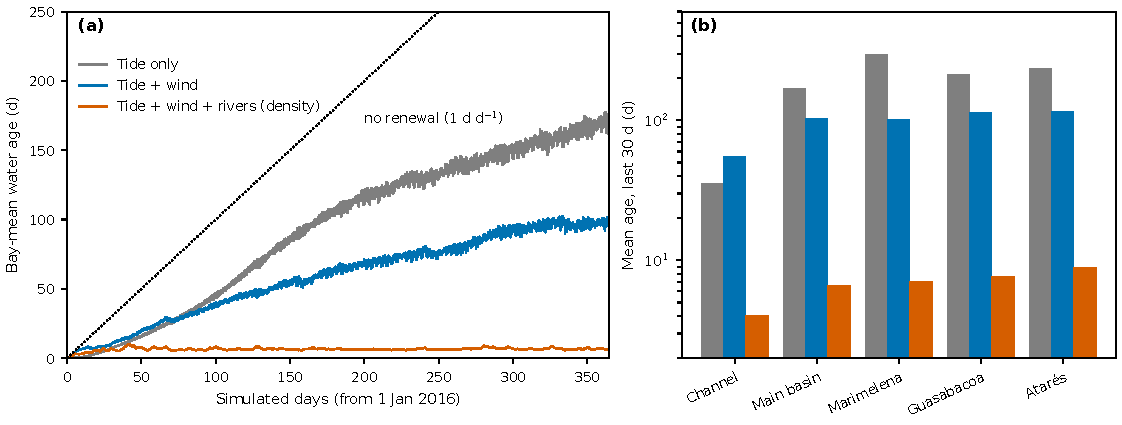
\includegraphics[width=\textwidth]{figuras/fig_mechanism.pdf}
\caption{Bay-mean water age in the three mechanism runs, 2016. (a) Daily series over one
year; the dotted line is the age of water that is never renewed. (b) Volume-weighted mean
age of each zone over the last 30 days (logarithmic axis); grey, tide only; blue, tide and
wind; orange, tide, wind and rivers.}\label{fig:mech}
\end{figure*}

\subsection{About a week across the ensemble, set mostly by the rivers}\label{sec:res-map}\label{sec:res-sobol}
Across the ensemble the bay is renewed in about a week, but not reliably faster
(Table~\ref{tab:ens}, Fig.~\ref{fig:ens}). The median bay-mean age is 7.8~days (5.6--10.4
between the 5th and 95th percentiles); it exceeds 7~days in 68\% of the members and 14~days
in none. The channel, the main basin, Guasabacoa and Atar\'es age in that order in every
member, from a median of 4.6~days in the channel to 10.5~days in Atar\'es, the only zone
where some members pass two weeks (11\%). At the surface, water older than a week is likely
almost everywhere except in the outer channel, while water older than two weeks appears only
towards the head of Atar\'es (Fig.~\ref{fig:ens}b,c).

\begin{table}[!t]
\centering\small
\caption{Mean water age (days) over the last 30 of 120 days in the ensemble: median and
P5--P95 over the 128 members of blocks A and B, and probability that the zone mean age
exceeds 7, 14 and 30 days.}\label{tab:ens}
\footnotesize\setlength{\tabcolsep}{4pt}
\begin{tabular}{@{}lrrrr@{}}
\toprule
Zone & Age (P5--P95) & $>7$~d & $>14$~d & $>30$~d\\
\midrule
Channel & 4.6 (3.2--6.4) & 0.02 & 0 & 0\\
Main basin & 7.7 (5.6--10.2) & 0.69 & 0 & 0\\
Marimelena & 8.1 (6.3--10.4) & 0.82 & 0 & 0\\
Guasabacoa & 9.1 (6.4--12.5) & 0.85 & 0 & 0\\
Atar\'es & 10.5 (7.3--14.6) & 0.96 & 0.11 & 0\\
Whole bay & 7.8 (5.6--10.4) & 0.68 & 0 & 0\\
\bottomrule
\end{tabular}
\end{table}

\begin{figure*}[!t]
\centering
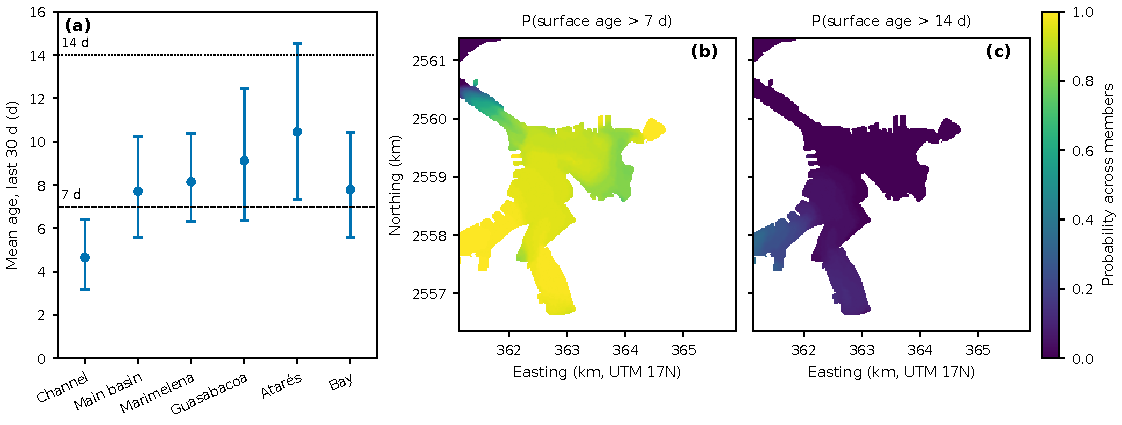
\includegraphics[width=\textwidth]{figuras/fig_ensemble.pdf}
\caption{Water age across the ensemble (128 members of blocks A and B, last 30 of 120
days). (a) Mean age of each zone: median and P5--P95; the dashed and dotted lines are the
7- and 14-day thresholds. (b, c) Probability across members that the surface age exceeds 7
and 14 days.}\label{fig:ens}
\end{figure*}

Most of the conclusions fixed in advance therefore hold (Table~\ref{tab:concl}). The order of
the zones, an age below one month and well below four months, and a channel whose surface
water is older than its bottom water, the signature of the estuarine circulation, are robust:
they hold in every member. Marimelena is older than the main basin in only 76\% of the
members, in keeping with its shifting place in the mechanism runs; an age above one week is
fragile, and ages above two weeks or one month are rejected.

\begin{table*}[!t]
\centering\small
\caption{Conclusions fixed before the results were computed (C, P: metrics protocol,
27 October 2026; R: tracer protocol, 8 November 2026) and their outcome. ``Holds in'' is the
fraction of the 128 members of blocks A and B, or the number of the four tracer cases. The
last column repeats the test with the air--sea heat flux and OISST temperature: in the
64 members of block A rerun with it, as fractions of the 64, for C1--C7 and P, and in
tracer case T3 for R1--R4 (Section~\ref{sec:res-robust}). Without the heat flux, the same 64
members give 49/64 for C3, 42/64 for P(age $>$ 7~d) and 0/64 for P(age $>$ 14~d). Case T1 failed the tracer-budget check of the protocol;
R1--R4 hold with both transport-solver tolerances (Section~\ref{sec:extra}).}\label{tab:concl}
\begin{tabular}{lp{9.6cm}rll}
\toprule
& Conclusion & Holds in & Class & With heat flux\\
\midrule
C1 & Mean age increases from channel to basin to Guasabacoa to Atar\'es & 1.00 & Robust & Robust (58/64)\\
C2 & Atar\'es is older than the channel & 1.00 & Robust & Robust (64/64)\\
C3 & Marimelena is older than the main basin & 0.76 & Fragile & Robust (64/64)\\
C4 & Guasabacoa and Atar\'es are older than the main basin & 1.00 & Robust & Robust (58/64)\\
C5 & Bay-mean age is below 30 days & 1.00 & Robust & Robust (64/64)\\
C6 & Bay-mean age is below 120 days (the ``four months'' of \citealt{JICA2004}) & 1.00 & Robust & Robust (64/64)\\
C7 & In the channel, surface water is older than bottom water (estuarine circulation) & 1.00 & Robust & Robust (64/64)\\
P & Bay-mean age exceeds 7 days & 0.68 & Fragile & Robust (63/64)\\
P & Bay-mean age exceeds 14 days & 0 & Rejected & Fragile (27/64)\\
P & Bay-mean age exceeds 30 days & 0 & Rejected & Rejected (0/64)\\
C8 & Input with the largest total Sobol index for the bay-mean age: river discharge & -- &
Reported & Discharge$^{a}$\\
\midrule
R1 & The water of each river is renewed in less than 7 days ($T_i < 7$~d) & 4 of 4 & Robust & Holds (T3)\\
R2 & River water is a smaller fraction of the volume of Atar\'es than of Guasabacoa & 4 of 4 & Robust & Holds (T3)\\
R3 & Most of the Luyan\'o and Mart\'in P\'erez water in the bay is in Guasabacoa and the
main basin ($>50$\% of $M_i$) & 4 of 4 & Robust & Holds (T3)\\
R4 & Most of the Tadeo water in the bay is in Marimelena ($>50$\% of $M_\mathrm{Tadeo}$) & 0 of 4 & Rejected & Fails (T3)\\
\bottomrule
\multicolumn{5}{l}{\footnotesize $^{a}$ Largest Spearman correlation with the bay-mean age
($\rho = -0.79$); the tidal amplitude factor, controlled for discharge, gives $-0.13$.}\\
\end{tabular}
\end{table*}

The unknown behind most of the remaining spread is easy to name (Fig.~\ref{fig:sobol}). River
discharge has a total Sobol index $S_T = 0.67$ (0.49--0.89) and a first-order index
$S_1 = 0.86$ (0.80--0.90) for the bay-mean age, and it leads in every zone ($S_T$
0.56--0.70). A long way behind come the chart-error field ($S_T$ 0.09--0.14) and, for the
whole bay, the wind direction (0.05) and the choice of survey (0.03). The dredging state,
the datum, the bottom drag, the wind speed and the tidal amplitude all have
$S_T \le 0.013$: they cannot be told apart from zero in this design, which is not the same
as being irrelevant. That $S_T$ falls below $S_1$ for discharge is estimator noise, since
$S_T \ge S_1$ in theory \citep{Saltelli2008} and the intervals overlap. The ranking does not
depend on the sample size: recomputed with 176 and 352 members ($N = 16$ and 32), discharge
keeps the largest $S_T$ (0.70 and 0.61) in the whole bay and in every zone
(Fig.~\ref{fig:sobolconv}), and a given-data estimate from the 128 members of blocks A and B
confirms it ($S_1 = 0.83$, against 0.12 for the 95th percentile of a permutation null).
With $N = 64$, the first-order indices of the minor inputs carry intervals of about
$\pm0.3$.

\begin{figure*}[!t]
\centering
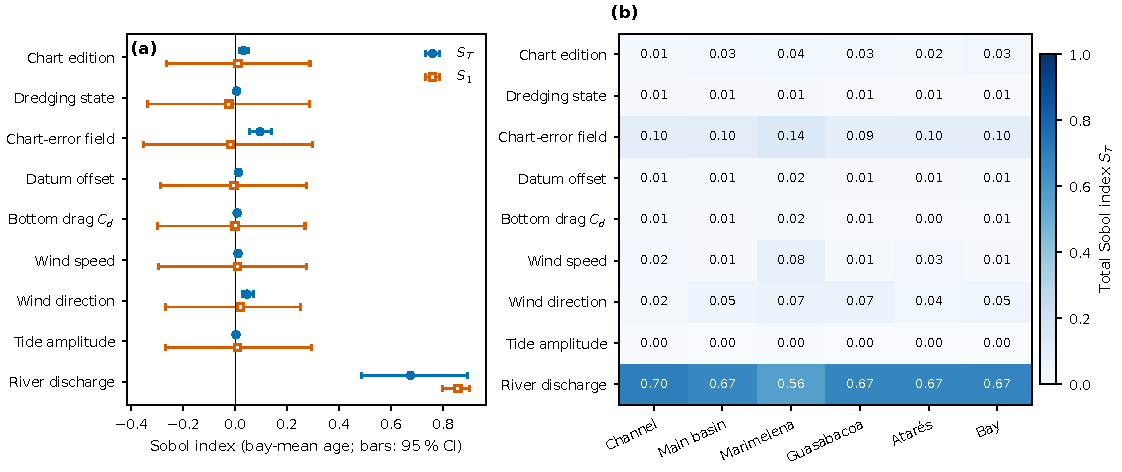
\includegraphics[width=\textwidth]{figuras/fig_sobol.pdf}
\caption{Sobol sensitivity of the mean water age (Jansen estimators, $N = 64$, 704
members). (a) First-order ($S_1$) and total ($S_T$) indices for the bay-mean age, with 95\%
bootstrap intervals (1000 resamples). (b) Total index of each input for each zone and the
whole bay.}\label{fig:sobol}
\end{figure*}

\subsection{The air--sea heat flux shifts the age as much as all sampled inputs together}\label{sec:res-robust}\label{sec:res-season}
All of this holds within the structure that the ensemble shares: density from salinity
alone, January--April 2016, and the 2002 river flows scaled by 0.25--2. Changing how
turbulence and vertical resolution are represented hardly matters (Table~\ref{tab:robust},
Fig.~\ref{fig:robS}). With the $k$--$\varepsilon$ closure, twice as many levels or ten times
more background mixing, the bay-mean age stays at 6.6--7.5~days, the channel keeps its older
surface water and the zones keep their order. The air--sea heat flux is another matter. In
the central member, with the ERA5 heat flux and the boundary fixed at 28~$^\circ$C, the
bay-mean age reaches 16.8~days and the surface--bottom contrast in the channel largely
disappears, although that boundary was up to 3.5~$^\circ$C too warm. With the daily OISST
temperature the age reaches 11.2~days over days 90--120 and is still rising
($+0.24$~d\,d$^{-1}$), while the channel keeps an older surface (10.0~days) than bottom
(6.6~days) and the zones keep their order.

The effect is not a peculiarity of one member (Fig.~\ref{fig:heat}b). Rerunning the 64
members of block A with the heat flux and the OISST boundary raises the bay-mean age in every
one of them: the median goes from 7.6~days (5.5--10.7 between the 5th and 95th percentiles)
to 13.2~days (8.3--18.4), with a paired median shift of 5.4~days. That is as large as the
5.3~days spanned by the P5--P95 range of the nine inputs in the same members, so one
structural choice moves the answer as far as all nine sampled inputs together. The shift is
largest in the members with the least river water and smallest in those with the most. The
oldest member reaches 24.4~days, and only 1 of the 64 members meets the equilibrium
criterion, against 59 of 64 without heat flux.

The robust conclusions survive (Table~\ref{tab:concl}, last column). The channel remains the
youngest zone and keeps its older surface water in every member, and the bay-mean age stays
below one month. The order of the zones (C1) and the older state of Guasabacoa and Atar\'es
relative to the main basin (C4) still hold in 58 of 64 members, robust but only just. River
discharge remains the dominant input (Spearman $\rho = -0.79$, against $-0.91$ without the
heat flux, and $-0.13$ for the tidal amplitude once discharge is controlled for). Three
verdicts change: Marimelena older than the main basin
(49/64 to 64/64) and an age above one week (42/64 to 63/64) become robust, and an age above
two weeks goes from rejected (0/64) to fragile (27/64). In the tracer case with the heat flux
(T3), R1--R3 hold and R4 fails, as in the other cases.

\begin{figure*}[!t]
\centering
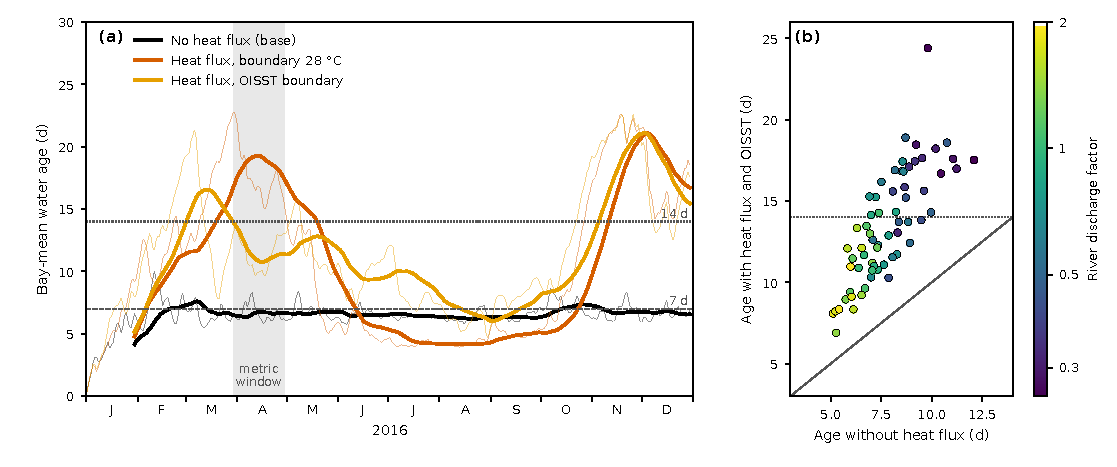
\includegraphics[width=\textwidth]{figuras/fig_heatflux.pdf}
\caption{Effect of the air--sea heat flux. (a) Bay-mean water age in the central member with
rivers through 2016, without heat flux and with the ERA5 heat flux and the open boundary at
28~$^\circ$C or at the daily OISST temperature (thin lines, daily values; thick lines,
trailing 30-day mean); the shaded band is the 30-day window of the ensemble metrics.
(b) Bay-mean age of the 64 members of block A (last 30 of 120 days) without and with the
heat flux and OISST temperature, coloured by the river discharge factor; the line is 1:1 and
the dotted line is 14~days.}\label{fig:heat}
\end{figure*}

A year-long view shows what the 120-day window hides (Fig.~\ref{fig:heat}a). Without heat
flux the bay-mean age settles at 6.57~days (drift $-0.03$~d\,d$^{-1}$) and averages 6.5~days
over the year. With the heat flux and OISST it averages 11.4~days, exceeds 14~days on 88 of
365 days (never without heat flux) and has 30-day means between 5.1 and 21.1~days; over the
last 30 days of the year it is 15.4~days and still rising ($+0.55$~d\,d$^{-1}$; channel
10.4~days, Atar\'es 18.2~days), and with the 28~$^\circ$C boundary it is 16.7~days, also
rising. The effect is seasonal. In a descriptive reading that was not part of the registered
one, the monthly means peak in November (21.0~days) and stay high from February to April
(11.4--13.9~days), but fall to 6.1~days in August, close to the 6.3~days of the base run; in
July--September the run with the 28~$^\circ$C boundary is the only configuration that renews
the bay faster than the base run. Because the age does not settle, the 30-day window of the
ensemble is one of several possible, and we do not extrapolate the 64-member results beyond
January--April.

What builds the age up and what resets it is harder to pin down. We compared the daily age
of the year-long runs with the bulk estimate of the net surface heat flux, using only rank
correlations because its annual balance and latent heat are probably biased. Cooling and the
growth of the age go together over 5-day blocks (Spearman $\rho = +0.32$ with OISST, $+0.51$
with the 28~$^\circ$C boundary, $-0.01$ without heat flux) and from month to month ($+0.75$
and $+0.66$, February--December). Once the wind is accounted for, however, the partial
correlation with OISST falls to $+0.14$, below the threshold of 0.25 fixed beforehand, so the
test is only partly supported: the age is highest in the months of net cooling and stronger
winds (October--March), and the two cannot be separated in a single year. The
surface--bottom density difference in the channel, which would separate them, was not
stored. \todo{EXPERIMENTO E2 --- resultado pendiente: factorial heat flux $\times$ wind over 2016}

\begin{table*}[!t]
\centering\small
\caption{Sensitivity of the density-driven circulation to the model structure: mean water
age (days) over days 90--120 of the central member with rivers.}\label{tab:robust}
\footnotesize\setlength{\tabcolsep}{4pt}
\begin{tabular}{lrrrrrr}
\toprule
& Base & $k$--$\varepsilon$ & 32 lev. & Diff.\,$\times10$ & Heat, 28\,$^\circ$C &
Heat, OISST\\
\midrule
Channel & 4.0 & 4.4 & 4.9 & 4.1 & 11.5 & 7.6\\
Main basin & 6.7 & 7.0 & 7.5 & 6.7 & 17.9 & 11.8\\
Marimelena & 7.0 & 7.1 & 7.5 & 7.1 & 19.3 & 12.9\\
Guasabacoa & 7.6 & 8.0 & 8.7 & 7.6 & 18.1 & 12.1\\
Atar\'es & 8.8 & 9.4 & 10.0 & 8.8 & 19.5 & 13.3\\
Whole bay & 6.6 & 6.9 & 7.5 & 6.6 & 16.8 & 11.2\\
Trend (d\,d$^{-1}$) & $+0.02$ & $+0.01$ & $+0.01$ & $+0.03$ & $-0.10$ & $+0.24$\\
Channel sfc./bot. & 6.6/1.8 & 6.7/2.1 & 7.5/2.3 & 6.6/1.9 & 14.2/10.6 & 10.0/6.6\\
\bottomrule
\end{tabular}
\end{table*}

\subsection{Where the river water goes}\label{sec:res-fate}
The water of each river leaves the bay within days (Fig.~\ref{fig:fate}). Its renewal time
$T_i$ is 1.7--2.5~days in the central case and 1.3--5.7~days over the four cases, the longest
being the Tadeo with a quarter of its discharge, so R1 holds everywhere; more discharge means
faster renewal, as expected when the rivers themselves drive the exchange. In five of the
twelve river--case pairs $M_i$ was still drifting, by $-2.3$ to $+1.5$\% per day, which adds
to the numerical uncertainty of $T_i$. The Luyan\'o and Mart\'in P\'erez water spreads from
the head of Guasabacoa into the main basin: 63--64\% and 67--69\% of it, respectively, lies
in Guasabacoa and the main basin in all four cases (R3). Atar\'es receives a smaller fraction
of river water than Guasabacoa in every case, but only by 6--11\% in relative terms (R2). The
Tadeo is the surprise. It enters on the shore of Marimelena, yet only 10--15\% of its water in
the bay stays there, against 44--48\% in the main basin, so R4 is rejected in all four cases.

\begin{figure*}[!t]
\centering
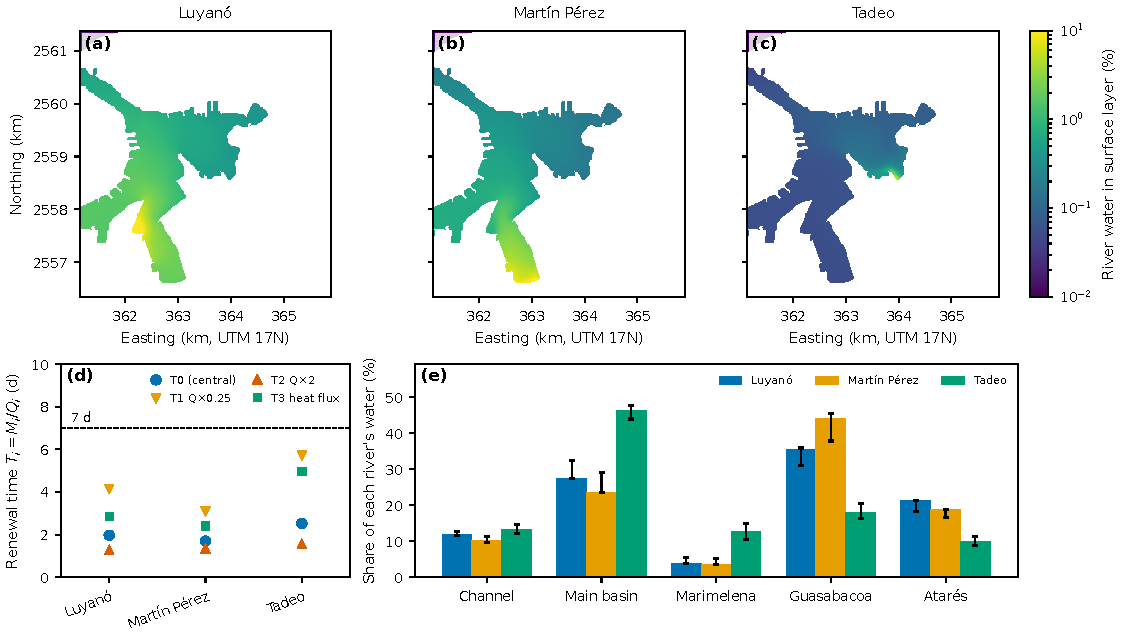
\includegraphics[width=\textwidth]{figuras/fig_rivers.pdf}
\caption{Water of each river in the bay. (a--c) Fraction of river water in the surface
layer, case T0, last 30 days: (a) Luyan\'o, (b) Mart\'in P\'erez, (c) Tadeo (logarithmic
scale). (d) Renewal time $T_i = M_i/Q_i$ of each river in the four cases; the dashed line
is the 7-day threshold of R1. (e) Share of the water of each river in the bay that lies in
each zone, case T0; bars show the range of the four cases.}\label{fig:fate}
\end{figure*}

\subsection{Sentinel-2 agrees, but so would chance}\label{sec:res-s2}
The surface fresh water of the run with rivers does correlate with the persistence of
turbidity anomalies, $\rho = 0.45$ (0.35--0.54) over 8908 pixels in 145 blocks, so the
registered prediction holds (Fig.~\ref{fig:s2}). The shift control takes the result away,
however: 5\% of the shifted satellite maps give correlations of 0.61 or more, and 16\% beat
the observed value ($p = 0.16$), so under the rule registered beforehand the agreement cannot
be told apart from spatial chance. The age fields of the runs with rivers, with tide and wind,
and with the tide alone behave the same way ($\rho$ = 0.46, 0.48 and 0.29;
$p$ = 0.15--0.28), and $\rho$ is positive in all 128 ensemble members (median 0.45, P5--P95
0.43--0.47), which says only that the pattern hardly depends on the inputs. Both maps simply
increase from the mouth towards the heads of the coves, and any field with that gradient
matches the satellite record. Sentinel-2 confirms that gradient and nothing more.

An exploratory pattern noticed after the test, a satellite signal at the head of Atar\'es,
where no modelled river enters, is discussed in Text~S2.

\begin{figure*}[!t]
\centering
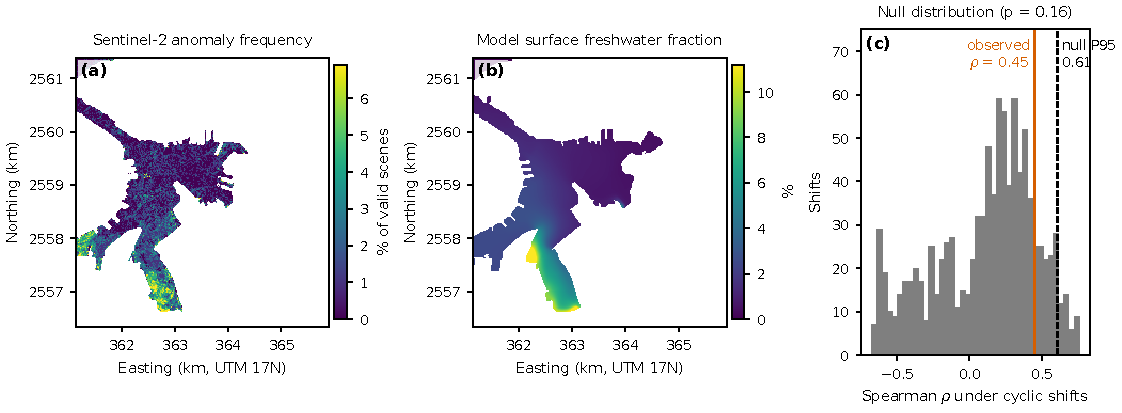
\includegraphics[width=\textwidth]{figuras/fig_sentinel2.pdf}
\caption{Comparison with Sentinel-2. (a) Frequency of positive turbidity anomalies,
2017--2025 (\% of valid scenes; companion study, \ph{link\_sentinel2}). (b) Modelled surface
freshwater fraction at 16:00~UTC, last 30 days of the mechanism run with rivers.
(c) Spearman $\rho$ between the two maps under 999 cyclic shifts of the satellite map by at
least 500~m; the solid line is the observed $\rho = 0.45$ and the dashed line the 95th
percentile of the shifts (0.61).}\label{fig:s2}
\end{figure*}

%======================================================================
\section{Discussion}\label{sec:discussion}
%======================================================================
\subsection{What the ensemble cannot see}\label{sec:disc-unc}
The conclusions that survive both the ensemble and the heat flux, the weak role of the tide,
the estuarine circulation in the channel, the ageing from the channel towards Atar\'es and a
renewal in weeks rather than months, are the ones we would defend without measurements. The
ones that change with the heat flux, whether the bay exceeds one or two weeks and whether
Marimelena is older than the main basin, depend on a process that needs its own data.

That contrast is the main lesson of the study. The P5--P95 range of the nine inputs,
5.6--10.4~days over the 128 members of blocks A and B, is the uncertainty that the ensemble
can see. One process that the ensemble leaves out shifts the median by as much again, raises
the age in every member tested and keeps it from settling, and nothing in the spread of the
ensemble hinted at it. This is the practical meaning of the distinction between input and
structural uncertainty \citep{Walker2003,Refsgaard2006,Gupta2012}: a Sobol analysis ranks the
uncertainties that the modeller has put into the design, and only tests of the structure
reveal those left outside it. Here the test was cheap, about $3.5\times10^3$ core-hours
against $5.4\times10^4$ for the ensemble, and we would argue that structural tests of this
kind belong next to any sensitivity analysis that is used to decide what to measure. For
Havana Bay, the safest summary therefore has two parts: in the dry season the bay is renewed
in about one week without the heat flux and in about two weeks, without settling, with it.
Either way it is weeks rather than months, faster where the river water flows out and slower
in Atar\'es.

The procedure itself can be repeated in other bays without surveys or gauges: digitise the
best historical charts, estimate their error from overlapping surveys, force the model with
global products, let a variance-based ensemble separate what the data can and cannot support
\citep{Pianosi2016,Razavi2021}, and test the conclusions again under the main structural
simplifications. The ranking it produced here, in which the century-old charts, the dredging
and the tide barely matter, a river discharge measured once in 2002 dominates the inputs and
the air--sea heat flux weighs as much as all of them, belongs to a small-tide bay with a
narrow channel in the dry season. The procedure does not.

\subsection{A thermal brake on the estuarine circulation?}\label{sec:disc-thermal}
The seasonal pattern suggests a mechanism, which we offer as a hypothesis because the runs
were not designed to test it. In bays with little river inflow, heating and cooling can set
the density contrast with the sea as much as fresh water does \citep{Largier2010}, and
shallow water that cools faster than the deeper water offshore drives an exchange of its own
\citep{Monismith2006,Doda2022}. In Havana Bay the two would compete. The river water makes the
bay lighter than the sea and drives the estuarine circulation, whereas winter cooling of the
shallow bay would make it denser and push the exchange the other way, weakening the
circulation and letting the age grow.

Four results fit this reading. The heat flux lengthens the age most in the months of net
cooling and hardly at all in August. It lengthens it most in the members with the least river
water, where the buoyancy that cooling has to overcome is weakest (Fig.~\ref{fig:heat}b).
With the boundary held at 28~$^\circ$C, warmer than the winter sea, the surface--bottom
contrast in the channel largely disappears (Table~\ref{tab:robust}), as expected if the two
circulations nearly cancel. And the same boundary is the only configuration that renews the
bay faster than the base run, in July--September, \prov{when the sea is usually warmer than
28~$^\circ$C} and the bay would then be lighter than the water entering it. One result does
not fit: once the wind is accounted for, the correlation between cooling and the growth of
the age falls below the threshold fixed beforehand, and winter is also the season of the
strongest winds. The decisive evidence, the density or temperature contrast between the bay
and the open boundary, was not stored; it can be recovered from the model and checked against
satellite thermal images (Section~\ref{sec:measure}). \todo{EXPERIMENTO E1 --- resultado
pendiente: monthly bay--boundary temperature contrast against the age anomaly}
\todo{EXPERIMENTO E3 --- resultado pendiente: Landsat 8/9 bay--sea temperature by season}

\subsection{Why the earlier estimates went wrong}\label{sec:jica}
Neither of the two simple estimates describes the bay, and for opposite reasons. The tidal
prism puts renewal at about three weeks, and the model falls on either side of it depending
on what drives the flow. With the tide alone the bay is much slower (166~days, still
rising), because nearly all the water that leaves on the ebb comes back and the real
return-flow factor is close to one \citep{Sanford1992}; with rivers and density it is much
faster, because the exchange is carried by a gravitational circulation that a prism does
not contain \citep{MacCready2010}. The estimate gets the diagnosis right, that the tide alone
does little, but in a small-tide bay behind a narrow channel it is a poor guide in both
directions.

The four months of the earlier report \citep{JICA2004} cannot be set directly against water
age, which counts river water as new water; the comparable quantity is the freshwater
flushing time. In the runs with full fields, fresh water makes up 1.1--1.2\% of the bay
volume (2.3--2.5\% at the surface), which gives $T_f \approx 1.8$--2.0~days, or 4.2~days
with the heat flux and the 28~$^\circ$C boundary, in line with the renewal times of the three
rivers (1.3--5.7~days). The gap with four months is therefore about a factor of 60: the river water leaves quickly
in the surface layer, and the bay-mean age is longer than $T_f$ only because it also follows
the sea water entering near the bottom. The report does not give its method, but with its
own volume of 47~hm$^3$, four months is what one obtains by dividing the bay volume by an
inflow of about 4.5~m$^3$\,s$^{-1}$, that is, by assuming no exchange with the sea; we cannot
confirm that this was the calculation. Even the largest structural effect we found raises the
bay-mean age only to about two weeks (24.4~days in the oldest of the 64 members, and 30-day
means never above 21.1~days over a full year), still about five times shorter.

\subsection{What to measure first, and what this study cannot say}\label{sec:measure}
Two measurements stand out, one for each kind of uncertainty. Among the inputs, river
discharge carries most of the variance of the age in every zone, and the
2.14~m$^3$\,s$^{-1}$ used here are a single set of 2002 values that leaves out sewage and
drains. The ranking is conditional on the ranges of Table~\ref{tab:params}, since the
discharge factor spans a factor of eight whereas the tide and wind factors span
$\pm$10--20\%; it shows which of the present uncertainties matter most, not which processes
do. Even so, gauging the three rivers and the main outfalls would reduce the uncertainty more
than any new survey of the bay, where only the chart error matters. For the structure, a
temperature and salinity record in the bay, with profiles in the channel, would constrain
the heat flux and show directly whether the estuarine circulation on which the robust
conclusions rest (C7) exists. Before any fieldwork, the thermal bands of Landsat~8 and 9,
which are public, could show whether the bay is colder than the adjacent sea in winter and
warmer in summer, as the hypothesis of Section~\ref{sec:disc-thermal} requires.

The study has other limits. The bathymetry comes from surveys more than a century old; the
dredging state and the chart error bound that uncertainty but do not remove it. The heat flux
was tested without a Sobol analysis, so we know that its effect grows as discharge falls but
not how it interacts with the other inputs, and the bulk heat-flux estimate used to read the
seasonal pattern is not the flux of the model. Net evaporation minus precipitation in the dry
season is roughly 0.1~m$^3$\,s$^{-1}$, about 5\% of the river inflow, although evaporation
can reverse the density contrast of shallow bays with little river flow \citep{Largier1997}.
The ensemble covers January--April 2016 only; wind explains little of its variance ($S_T$
0.011 for speed and 0.046 for direction), so the year is unlikely to change its conclusions,
but the heat-flux tests depend on that year's temperatures. The transport-solver tolerance
adds about 5\% of numerical uncertainty to water age (a $10^5$-fold stricter tolerance raised
the bay-mean age by 5\%, lowered $T_f$ by 3\% and left the Sentinel-2 $\rho$ and R1--R4
unchanged), and the discharge through the channel cannot be used as a result because of
intermittent high-frequency bursts of unexplained origin. Above all, no local observation
constrains the model: the results describe what public data allow, not a calibrated
reconstruction of the bay.

%======================================================================
\section{Conclusions}\label{sec:conclusions}
%======================================================================
With public data alone, a good deal can be said about the renewal of Havana Bay, and it can
be said with known confidence. The tide by itself leaves a bay-mean age of 166~days and the
wind 97~days; it is the density contrast of 2~m$^3$\,s$^{-1}$ of river water, acting through
an estuarine circulation that survives changes of turbulence closure, resolution and mixing,
that brings it down to 6.6~days. Across a 704-member ensemble of the poorly known inputs the
bay-mean age is about a week (median 7.8~days, P5--P95 5.6--10.4) and never above 14~days,
water gets older from the channel to Atar\'es in every member, and river discharge, not the
nineteenth-century charts, the dredging or the tide, controls most of the spread
($S_T = 0.67$, stable from $N = 16$ to 64). The water of each river leaves within six days,
and the freshwater flushing time of about two days is some 60 times shorter than the four
months of the earlier report.

The air--sea heat flux, which the ensemble leaves out, changes the answer as much as all nine
inputs together. In the 64 members rerun with it, the median January--April age rises from
7.6 to 13.2~days, in every member, and no longer settles; over a year the effect is strongest
from November to April and nearly vanishes in August, while the order of the zones and the
estuarine circulation survive. In the dry season the bay is therefore renewed in about one
week without the heat flux and about two weeks with it: in weeks, not months. Whether winter
cooling brakes the estuarine circulation remains a hypothesis. To narrow the answer, the
rivers and outfalls should be gauged first, and a temperature and salinity record in the bay
is the first measurement for the model structure. More generally, a sensitivity analysis
says which of the chosen inputs matter; only tests of the model structure say whether the
right ones were chosen.

%======================================================================
\section*{Software availability}
\noindent\textit{Name of software:} \ph{nombre\_repositorio}\par
\noindent\textit{Description:} Scripts that download the public inputs, digitise the
charts, build the bathymetry and mesh, generate and run the 704-member SCHISM ensemble on
a Slurm cluster, and post-process the results, with the three analysis protocols.\par
\noindent\textit{Developers:} Alex M. Rivera-Rivera et al.\par
\noindent\textit{Contact:} alex.rivera.rivera@ulb.be\par
\noindent\textit{Language:} Python, Bash, Fortran (SCHISM, Apache~2.0)\par
\noindent\textit{Software required:} SCHISM (commit 09f407e8), Python, Bash, Slurm\par
\noindent\textit{Hardware required:} a Slurm cluster for the ensemble (about 76 core-hours
per member)\par
\noindent\textit{Availability and cost:} free and open source, MIT licence\par
\noindent\textit{Source code:} \ph{link\_repositorio}

\section*{Data availability}
All inputs are public (Table~\ref{tab:data}); each download is recorded with its date in
the repository (\ph{link\_repositorio}). The repository also holds the post-processed
outputs of the ensemble, the mechanism, structural and tracer runs, the design of the
ensemble, and the three analysis protocols with their dated version history. The commits
that fixed the protocols are 773b9fb (Sentinel-2 comparison, 21 October 2026), 231696a (its
shift control, 26 October), 4564b7e (ensemble metrics, committed on 26 October and approved
on 27 October) and 3907fd7 (river tracers, 8 November). The readings of the later heat-flux tests were fixed in 7c74c13 (year-long runs,
14 November) and a553d4d (64-member rerun and heat-flux proxy, 16 November); an earlier
16-member subset (58d3d54, 15 November) gave the same three changes of class. The Sentinel-2 turbidity product is
not part of it: its processing and its definition of a turbidity anomaly are described in a
companion study, with its own repository (\ph{link\_sentinel2}).

\section*{Declaration of competing interest}
The authors declare that they have no known competing financial interests or personal
relationships that could have appeared to influence the work reported in this paper.

\section*{Funding}
This work was supported by ARES, with funding from the Belgian Development Cooperation,
through the project ``In situ monitoring of water quality in Cuban bays: creating and
promoting the use of a scientific toolbox''. A.C. and S.C.N. acknowledge funding from the
European Union's Horizon Europe research and innovation programme under grant agreement
No.~101181363 (BioDiMoBot).

\section*{Declaration of generative AI and AI-assisted technologies in the manuscript
preparation process}
During the preparation of this work the authors used Claude (Anthropic) and ChatGPT
(OpenAI) to check numerical consistency, to help write the code that draws the figures, and
to review and edit the language. After using these tools, the authors reviewed and edited
the content as needed and take full responsibility for the content of the published
article.

\section*{Acknowledgements}
Computational resources have been provided by the Consortium des \'Equipements de Calcul
Intensif (C\'ECI), \linebreak[1] funded by the Fonds de la Recherche Scientifique de Belgique
(F.R.S.-FNRS) under Grant No.\ 2.5020.11 and by the Walloon Region. All simulations
were run on the Lemaitre4 cluster of C\'ECI.

\printcredits

\bibliographystyle{cas-model2-names}
\bibliography{referencias}

%======================================================================
% Supplementary material: to be submitted as a separate file.
\clearpage
\onecolumn
\section*{Supplementary material}
\setcounter{figure}{0}
\renewcommand{\thefigure}{S\arabic{figure}}
\renewcommand{\theHfigure}{S\arabic{figure}}
\setcounter{table}{0}
\renewcommand{\thetable}{S\arabic{table}}
\renewcommand{\theHtable}{S\arabic{table}}

\begin{figure}[!h]
\centering
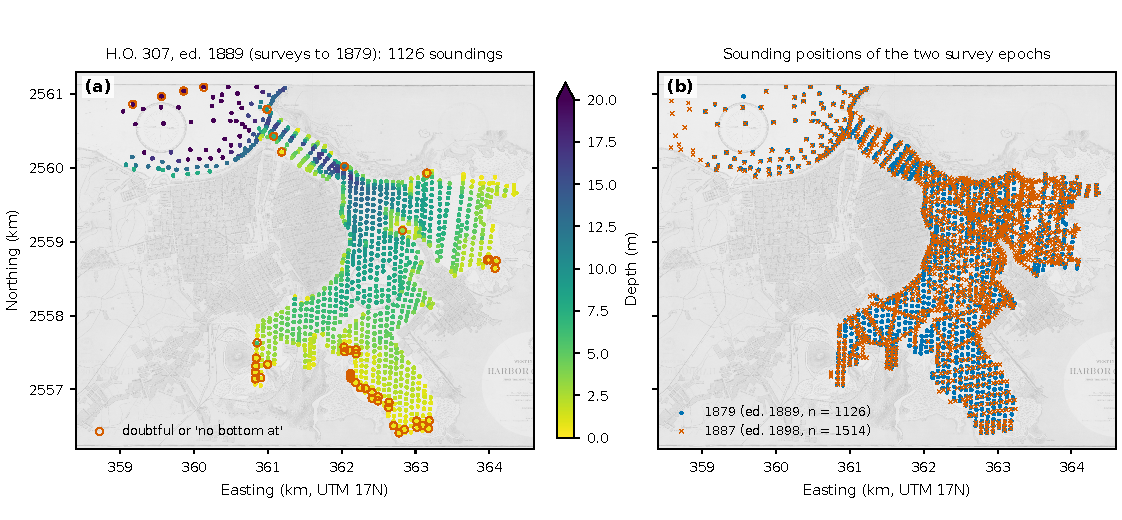
\includegraphics[width=\textwidth]{figuras/figS_soundings.pdf}
\caption{Digitised soundings of chart No.~307. (a) The 1126 soundings of the 1889 edition
(surveys to 1879), coloured by depth; circles mark doubtful readings and ``no bottom at''
entries. (b) Positions of the 1879 (1889 edition, 1126) and 1887 (1898 edition, 1514)
soundings. The 1887 soundings are drawn on the 1889 chart, printed from the same
plate.}\label{fig:soundings}
\end{figure}

\begin{figure}[!h]
\centering
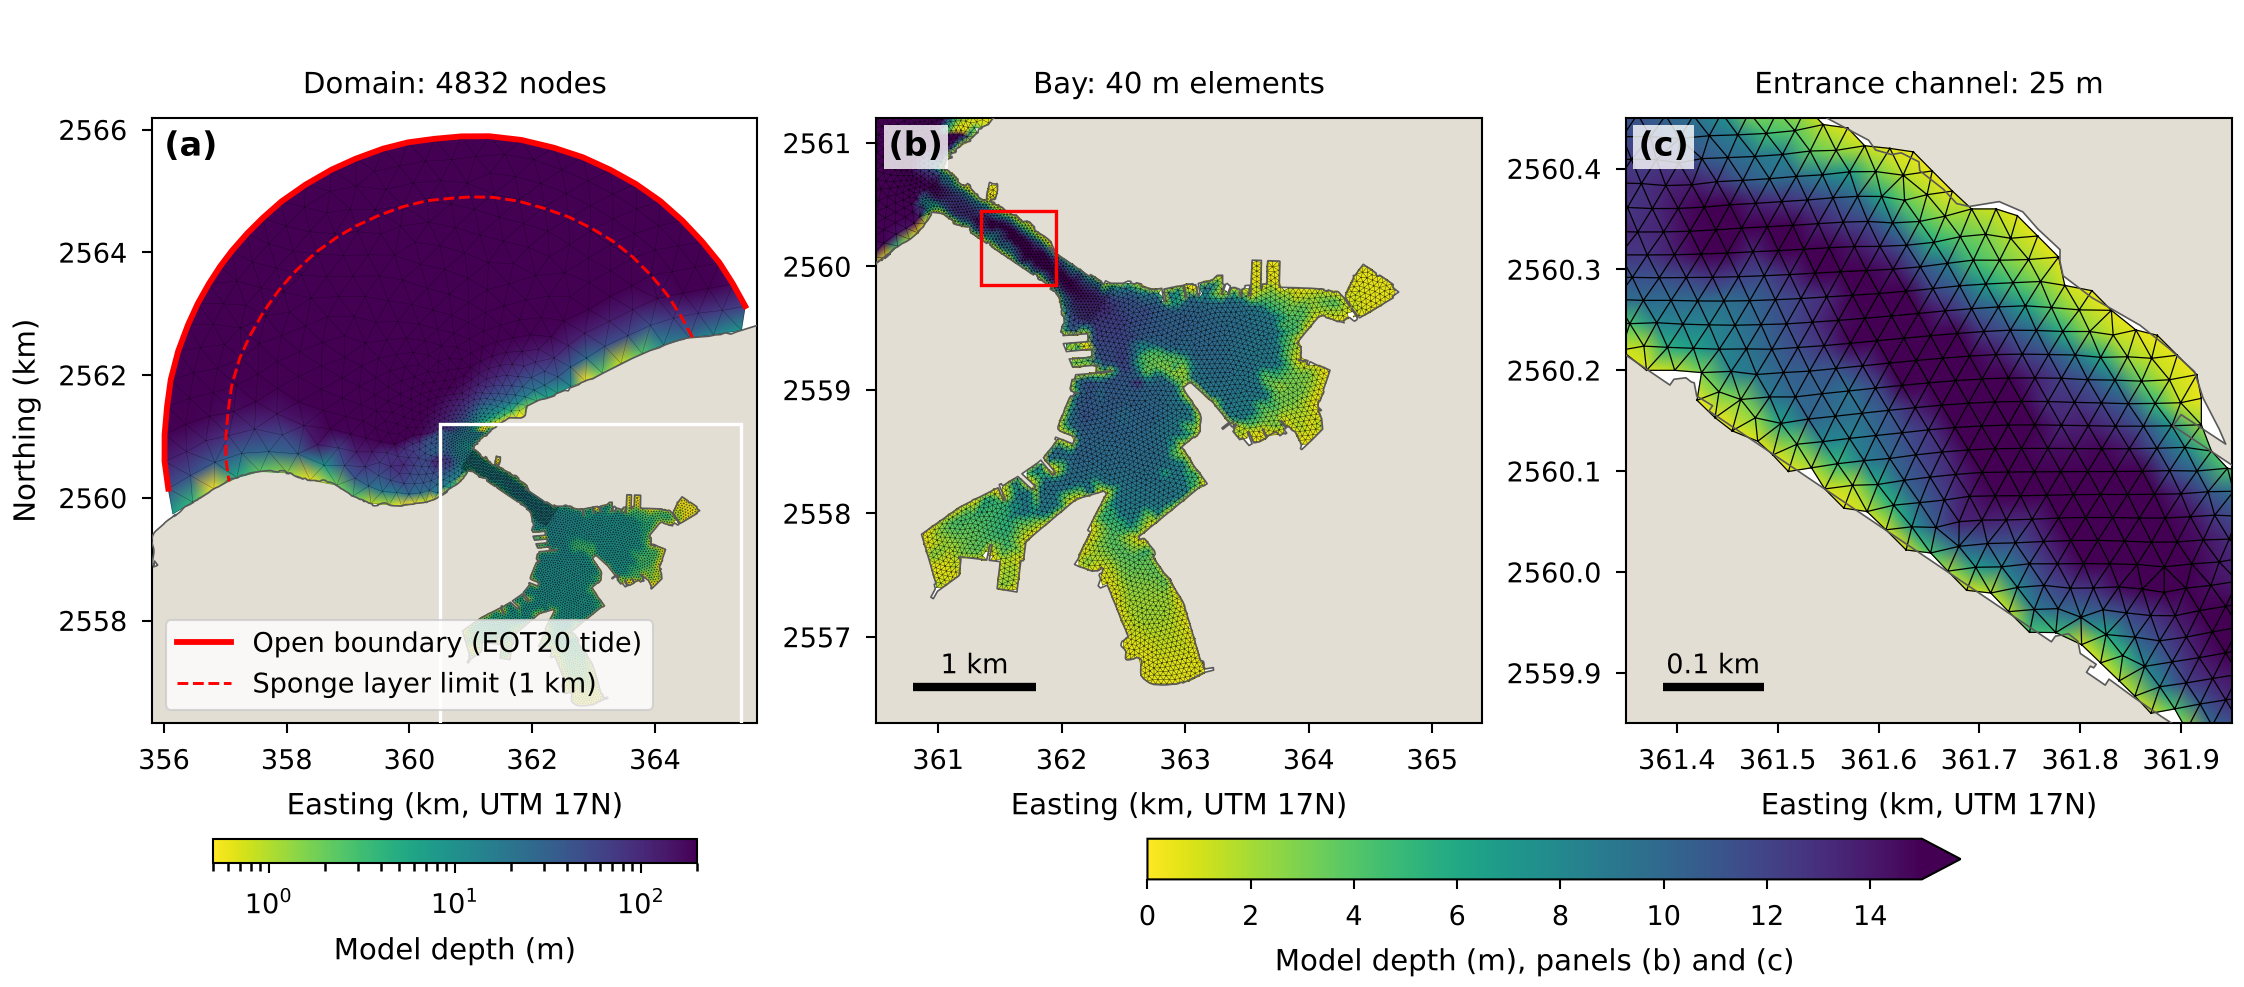
\includegraphics[width=\textwidth]{figuras/fig03_mesh.png}
\caption{Model mesh (4832 nodes, 8941 triangles), coloured by model depth. (a) Whole domain,
with the open boundary forced by the EOT20 tide and the inner limit of the 1~km sponge
layer. (b) The bay, with 40~m elements. (c) The entrance channel, with 25~m
elements.}\label{fig:mesh}
\end{figure}

\begin{figure}[!h]
\centering
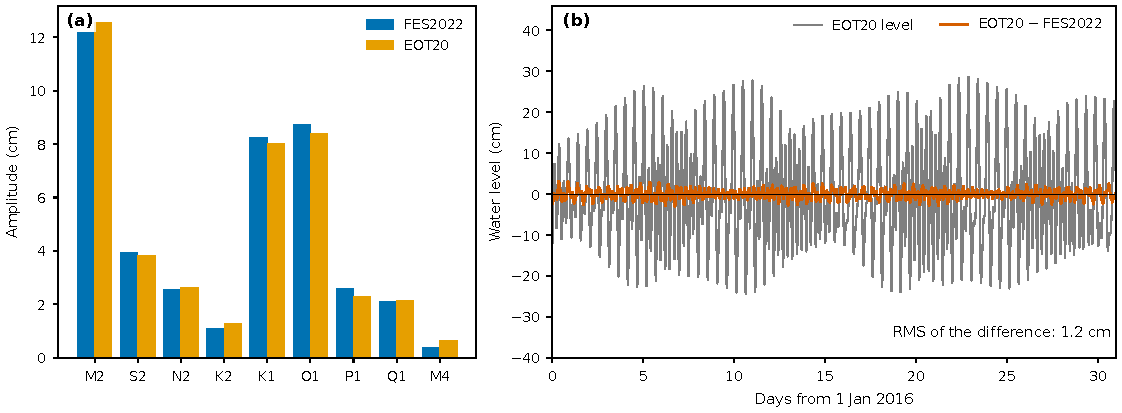
\includegraphics[width=\textwidth]{figuras/fig_tide.pdf}
\caption{Tide off the bay mouth. (a) Amplitudes of nine constituents in FES2022 and EOT20.
(b) Water level predicted with EOT20 and its difference from FES2022, January 2016 (RMS
1.2~cm).}\label{fig:tide}
\end{figure}

\begin{table}[!h]
\centering\small
\caption{Inputs of the Monte Carlo tidal-prism estimate (Section~\ref{sec:eval}), each drawn
from a triangular distribution ($2\times10^5$ samples). The tide is not a distribution: each
sample takes a real day of a year synthesised from the nine EOT20 constituents off the
mouth.}\label{tab:prismS}
\begin{tabular}{llrrrl}
\toprule
Input & Unit & Minimum & Mode & Maximum & Basis\\
\midrule
Bay area & km$^2$ & 4.7 & 4.91 & 5.2 & OpenStreetMap coastline\\
Mean depth & m & 5.2 & 6.2 & 7.3 & Charts, as surveyed to dredged (Section~\ref{sec:bathy})\\
Channel width & m & 220 & 220 & 280 & Harbour pilots, 220--330~m \citep{Practicos2018}\\
Channel section depth & m & 9.0 & 11.0 & 12.8 & 12.8~m axis, shallower margins\\
Return-flow factor $\beta$ & -- & 0.3 & 0.6 & 0.85 & Assumed\\
River inflow & m$^3$\,s$^{-1}$ & 1.0 & 2.14 & 5.0 & 2002 values \citep{JICA2004}, plus sewage\\
\bottomrule
\end{tabular}
\end{table}

\begin{figure}[!h]
\centering
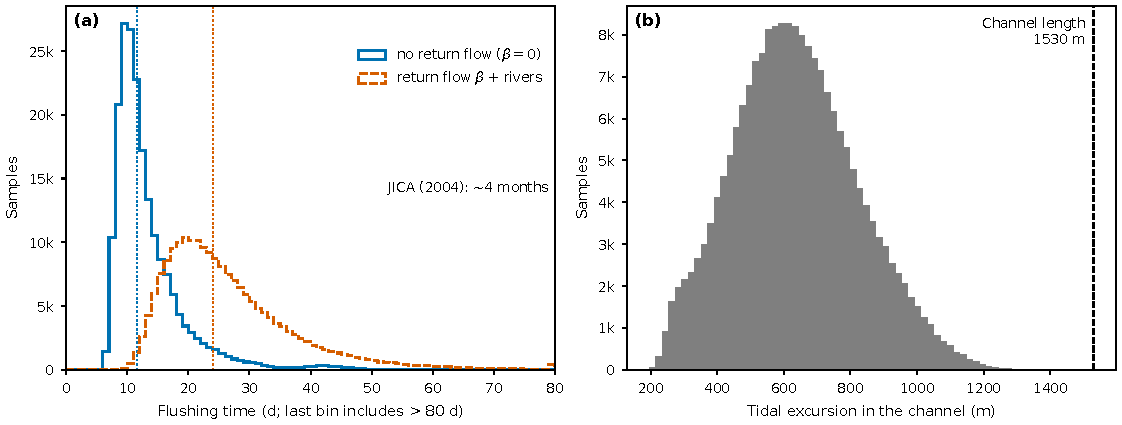
\includegraphics[width=\textwidth]{figuras/fig_prisma.pdf}
\caption{Monte Carlo tidal-prism estimate ($2\times10^5$ samples). (a) Flushing time without
return flow ($\beta = 0$) and with return flow and rivers; the dotted lines mark the
medians; the label marks the earlier estimate of about four months \citep{JICA2004}, far beyond the axis.
(b) Tidal excursion in the channel against the channel length of 1530~m.}\label{fig:prisma}
\end{figure}

\subsection*{Text S1. Tracer budget check}
The sum of the three river tracers must match the fresh water derived from salinity within
5\% of the bay inventory. The mismatch was 5.4\% in case T1, 2.2\% in T0, 0.5\% in T2 and
0.6\% in T3. We could not trace it to the flux limiter, the source injection or the
restarts. Tightening the transport-solver tolerance by five orders of magnitude moved it in
either direction (T0, 4.4\%; T1, 1.7\%; T2, 8.5\%; T3, 5.8\%), changed $T_i$ by $-21$ to
$+24$\%, which stays below 7~days, and did not change whether R1--R4 hold in any case. The
cause remains unidentified, and neither tolerance is the correct one.

\subsection*{Text S2. Sentinel-2 comparison}
We keep pixels that are water in both masks, lie at least two pixels from the coast (a
two-step erosion of the water mask, which keeps pixels whose centre is at least 44.7~m from
the nearest land pixel) and have at least 50 valid scenes (of the 113 scenes accepted out of
637 acquisitions). Model fields are interpolated to the 20~m grid of the satellite study; the
16:00~UTC output is the nearest to the Sentinel-2 overpass (16:16--16:17~UTC). The block
bootstrap uses 200~m~$\times$~200~m blocks and 1000 resamples. A secondary test uses the
surface age of the runs without rivers.

One pattern was noticed only after the test and is reported as exploratory: the satellite
frequency is highest towards the heads of the Guasabacoa and Atar\'es coves, and only the
former has a modelled river. The diagnostics of the companion study do not settle the cause.
In Guasabacoa the signal behaves like land adjacency \citep{Sterckx2011}, and in Atar\'es
piers lie 30--52~m away, which may point to berthed vessels; discharges missing from
OpenStreetMap and from the 2002 values, or resuspension in shallow water, are not excluded,
but the satellite data do not support them either. The modelled rivers cannot explain it,
since they put a little less of their water into Atar\'es than into Guasabacoa (R2).

\subsection*{Text S3. Computation and numerical behaviour of the ensemble}
Each member ran on seven cores, four for computation and three for output, and advanced in
20-day segments chained by hot-starts, which change the summary metrics by at most 0.01\%.
A 20-day segment takes 0.65--9~h of wall time (median 1.6~h); the cost of 76 core-hours per
member was estimated from 484 members. The heat-flux runs took about $3.1\times10^3$
core-hours for the 64 members and about 380 for the three year-long runs. The largest model speeds are spurious and do not
affect the results (Fig.~\ref{fig:boundary}). In 94\% of the members the maximum
depth-averaged speed (median 6.0~m\,s$^{-1}$) sits on the open boundary, 4--5~km from the
mouth, where the model depth is capped at 200~m. These speeds did not appear in a 10-day
rerun of the central member (maximum 1.8~m\,s$^{-1}$ in the same region), and we did not
isolate their cause; they are capped by the velocity limiter of SCHISM
(5~m\,s$^{-1}$ per component). Inside the bay, 68 members exceed 3~m\,s$^{-1}$ at a few
nodes only 0.3--0.5~m deep, where SCHISM caps the velocity. Neither is related to the
bay-mean age (Spearman $\rho = -0.07$ and $-0.04$), and removing the 15 such members of
blocks A and B changes no class (bay-mean age 7.73 instead of 7.78~days).

\begin{figure}[!h]
\centering
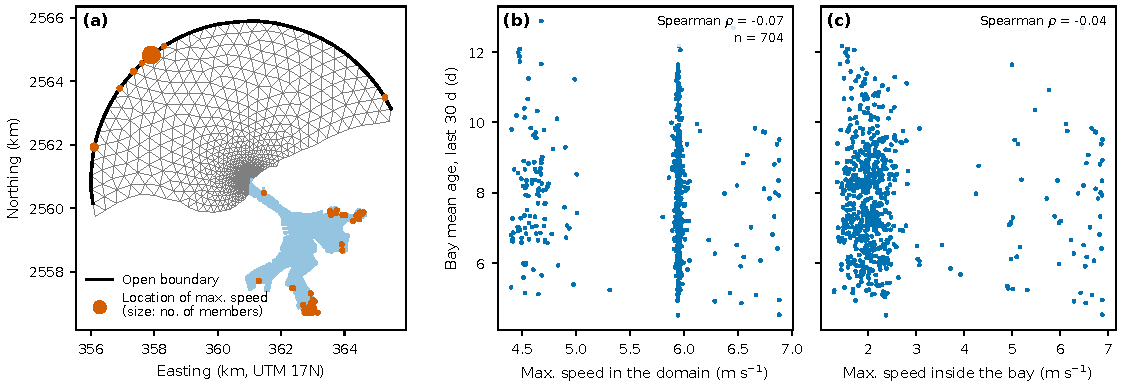
\includegraphics[width=\textwidth]{figuras/figS_boundary.pdf}
\caption{Spurious velocities in the 704 members. (a) Location of the maximum
depth-averaged speed of each member (symbol size: number of members). (b) Bay-mean age
against the maximum speed in the domain. (c) Bay-mean age against the maximum speed inside
the bay.}\label{fig:boundary}
\end{figure}

\begin{figure}[!h]
\centering
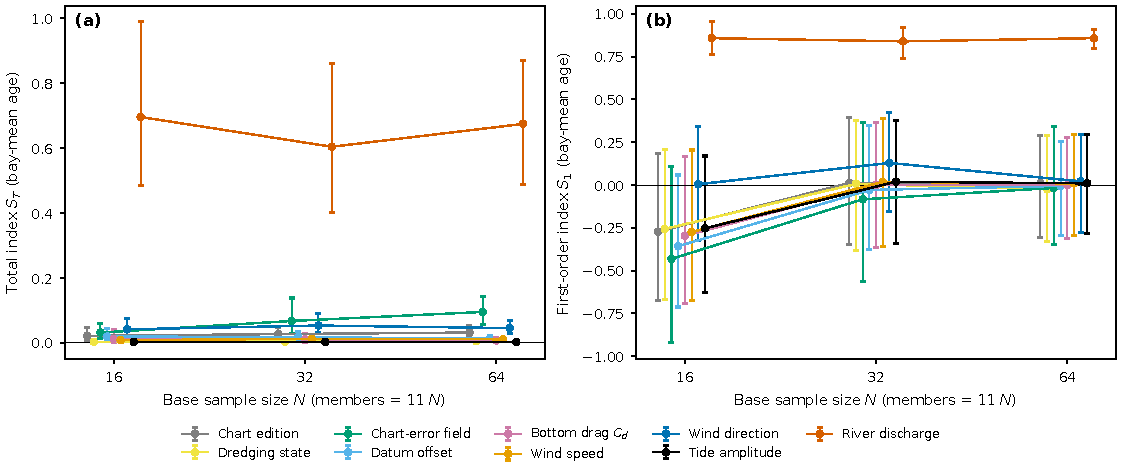
\includegraphics[width=\textwidth]{figuras/figS_sobol_convergence.pdf}
\caption{Convergence of the Sobol indices of the bay-mean age with the base sample size
$N$ (Jansen estimators on the first $N$ rows of each Saltelli block; members $= 11N$).
(a) Total indices $S_T$ and (b) first-order indices $S_1$ of the nine inputs, with 95\%
bootstrap intervals. River discharge has the largest $S_T$ at every $N$ (0.70, 0.61 and 0.68
for $N = 16$, 32 and 64) and in every zone (0.46--0.72), with $S_1 = 0.84$--0.86; the
chart-error field ranks second for $N = 32$ and 64 and swaps places with the wind direction
for $N = 16$, within overlapping intervals. In a given-data estimate from the 128 members of
blocks A and B (eight quantile bins, permutation null), only the bottom drag among the other
continuous inputs slightly exceeds its null (0.13 against 0.105), as expected by chance among
seven tests and consistent with its $S_T$ of 0.007.}\label{fig:sobolconv}
\end{figure}

\begin{figure}[!h]
\centering
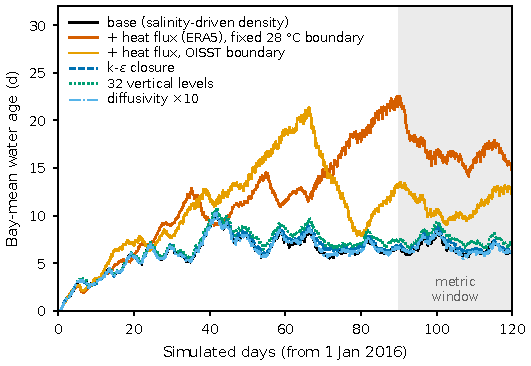
\includegraphics[width=0.6\textwidth]{figuras/fig_robustness.pdf}
\caption{Bay-mean water age in the central member with rivers over the first 120 days of
2016, under changes of model structure: base (salinity-driven density), $k$--$\varepsilon$
closure, 32 vertical levels, ten times larger background diffusivity, and the ERA5 air--sea
heat flux with the open boundary fixed at 28~$^\circ$C or at the daily OISST temperature.
The shaded band is the 30-day window of the metrics.}\label{fig:robS}
\end{figure}

\end{document}
